%LaTeX template : http://systbio.org/files/SB_LaTeX_Template_txt_extension.txt
%Author instructions: http://www.oxfordjournals.org/our_journals/sysbio/for_authors/ms_preparation.html

%NC: Supp material - add the actual table and figures for each thing. Also BE CONSISTENT. Is it Section 1 or S1? I'd go with S1 (which stands for Supp Mat 1 not section 1 really.). Normally you also refer to supplemental tables and figures as Table S1 etc. to distinguish between those in the main text. Check how Syst Biol does it.

\documentclass[12pt,letterpaper]{article}

%Packages
\usepackage{pdflscape}
\usepackage{fixltx2e}
\usepackage{textcomp}
\usepackage{fullpage}
\usepackage{natbib}
\usepackage{float}
\usepackage{latexsym}
\usepackage{hyperref}
\usepackage{url}
\usepackage{hyperref}
\usepackage{epsfig}
\usepackage{graphicx}
\usepackage{amssymb}
\usepackage{amsmath}
\usepackage{bm}
\usepackage{array}
\usepackage[version=3]{mhchem}
\usepackage{ifthen}
\usepackage{caption}
\usepackage{hyperref}
\usepackage{amsthm}
\usepackage{amstext}
\usepackage{enumerate}
\usepackage[osf]{mathpazo}
\pagenumbering{arabic}

%Pagination style and stuff
\linespread{1.66}
\raggedright
\setlength{\parindent}{0.5in}
\setcounter{secnumdepth}{0} 
\renewcommand{\section}[1]{%
\bigskip
\begin{center}
\begin{Large}
\normalfont\scshape #1
\medskip
\end{Large}
\end{center}}
\renewcommand{\subsection}[1]{%
\bigskip
\begin{center}
\begin{large}
\normalfont\itshape #1
\end{large}
\end{center}}
\renewcommand{\subsubsection}[1]{%
\vspace{2ex}
\noindent
\textit{#1.}---}
\renewcommand{\tableofcontents}{}
\bibpunct{(}{)}{;}{a}{}{,}

%---------------------------------------------
%
%       START
%
%---------------------------------------------

\begin{document}
%\modulolinenumbers[1]     % Line numbering on every line

%Running head
\begin{flushright}
Version dated: \today
\end{flushright}
\bigskip
\noindent RH: Missing data and topology in total evidence approach

\bigskip
\medskip
\begin{center}

\noindent{\Large \bf Effect of missing data on topological inference using a total evidence approach}

\bigskip

\noindent {\normalsize \sc Thomas Guillerme$^1$$^,$$^2$, and Natalie Cooper$^1$$^,$$^2$}\\
\noindent {\small \it 
$^1$School of Natural Sciences, Trinity College Dublin, Dublin 2, Ireland;\\
$^2$Trinity Centre for Biodiversity Research, Trinity College Dublin, Dublin 2, Ireland;}\\
\end{center}
\medskip
\noindent{\bf Corresponding author:} Thomas Guillerme, School of Natural Sciences, Trinity College Dublin, Dublin 2, Ireland; E-mail: guillert@tcd.ie; Fax: +353 1 6778094; Tel: +353 1 896 2571.\\
\vspace{1in}

%---------------------------------------------
%
%       ABSTRACT
%
%---------------------------------------------

\newpage
\begin{abstract}
Living species represent only a small proportion of all species that have ever lived. Ignoring fossil taxa may therefore lead to misinterpretation of macroevolutionary patterns and processes such as trends in species richness, biogeographical history or paleoecology. This fact has led to an increasing consensus among scientists that both living and fossil taxa must be included in macroevolutionary studies. One approach called Total Evidence, uses molecular data from living taxa and morphological data from both living and fossil taxa to infer phylogenies with both living and fossil taxa at the tips. Although the Total Evidence approach seems very promising, it requires a lot of data and is therefore likely to suffer from missing data issues which may affect its ability to infer correct phylogenies.

In this study we assess the effect of missing data on tree topologies inferred from Total Evidence matrices. Using simulations we investigate three major factors that directly affect the completeness of the morphological part of the matrix: (1) the proportion of living taxa with no morphological data, (2) the amount of missing data in the fossil record, and (3) the overall number of morphological characters in the matrix. 

% NC: This needs changing to reflect what we decided to focus on, i.e. our recommendations. We don't want to lead with the methods thing. The two previous paragraphs are fine and just need tightening up a bit
We find that, when using a clade conservative metric such as Robinson-Foulds distance, Bayesian consensus trees recovers the right topology better than Maximum Likelihood or than a subset of Bayesian posterior tree distributions and this regardless of the amount of missing data (minimal tree similarity of 0.69 in the worst scenario). Regarding the data, good topological recovery is not related to the amount of missing data \textit{per se} but to the amount of data overlap. The two factors that influences the most this data overlap are the parameters 1 (proportion of coded living taxa) and 3 (number of morphological characters).
\end{abstract}

\noindent (Keywords: missing data, Total Evidence, Bayesian, Maximum Likelihood, topology)\\

\vspace{1.5in}

\newpage 

%---------------------------------------------
%
%       INTRODUCTION
%
%---------------------------------------------

\section{Introduction}

Although most species that have ever lived are now extinct \citep{novacek1992ext,raup1993extinction}, the majority of macroevolutionary studies focus solely on living species \citep[e.g.][]{meredithimpacts2011,jetzthe2012}. Ignoring fossil taxa may lead to misinterpretation of macroevolutionary patterns and processes such as the timing of diversification events \citep[e.g.][]{pyrondivergence2011}, relationships among lineages \citep[e.g.][]{manosphylogeny2007} or niche occupancy \citep[e.g.][]{pearmanniche2008}. This has led to increasing consensus among evolutionary biologists that fossil taxa should be included in macroevolutionary studies \citep{jacksonwhat2006,quentaldiversity2010,dietlconservation2011,slaterunifying2013,fritzdiversity2013}. However, to do this we need to be able to place living and fossil taxa into the same phylogenies; a task that remains difficult despite recent methodological developments \citep[e.g.][]{pyrondivergence2011,ronquista2012,BEASTmaster}.

Up to now, three main approaches have been used to place both living and fossil taxa into phylogenies. These approaches differ mainly in whether they treat fossil taxa as tips or as nodes in the phylogeny, and in which part of the available fossil data is used (i.e. the age of the fossil only or both its age and morphology). Classical cladistic methods use matrices containing morphological data from both living and fossil taxa and treat each taxon as a tip in the phylogeny. Relationships among the taxa are then inferred using optimality criteria such as maximum parsimony \citep{simpson1945}. This approach is commonly used by paleontologists but it ignores the additional molecular data available from living species and does not allow use of probabilistic methods for dealing with phylogenetic uncertainty. Neontologists, on the other hand, more commonly use probabilistic approaches (e.g. Maximum Likelihood or Bayesian methods) based on matrices containing only molecular data from living species. Because fossil taxa do not usually have available DNA, fossils are used as nodes rather than tips in these phylogenies and their occurrence dates are used to time calibrate phylogenies \citep{zuckerkandl1965}. There have been great improvements in the theory and application of these two approaches \citep[e.g.][]{bapsta2013,stadlerdating2013,heaththe2013} as well as much debate about the "best" approach to use \citep[e.g.][]{spencerefficacy2013,wrightbayesian2014}. However neither approach uses all the available data.

A final approach, known as the Total Evidence method, uses matrices containing molecular data from living taxa and morphological data from both living and fossil taxa \citep{eernissetaxonomic1993}. This approach treats every taxon as a tip in the phylogeny, uses the occurrence age of the fossils to time calibrate the phylogeny (known as Tip-Dating; \citealt{ronquista2012}), and allows the use of probabilistic methods for estimating phylogenetic uncertainty \citep{ronquista2012}. Total Evidence methods have been successfully applied to empirical data \citep[e.g.][]{pyrondivergence2011,ronquista2012,schragocombining2013,slaterphylogenetic2013,beckancient2014}, and are becoming an increasingly popular way of adding fossil taxa to phylogenies. However, although the Total Evidence approach seems very promising, there is one big drawback in using this approach: it requires a lot of data that can be difficult (or impossible) to collect. The morphological data for living taxa are rarely collected when molecular data are available (e.g. \citealt{O'Leary08022013} \textit{vs.} \citealt{meredithimpacts2011}), and for fossil taxa, data can only be collected from features preserved in the fossil record (for example, in vertebrates, the hardest parts of the skeleton are more often preserved than soft parts; \citealt{sansomfossilization2013}). Therefore Total Evidence matrices are likely to contain a lot of missing data that may affect the method's ability to infer correct topologies, branch lengths and support values \citep{salamin2003}. 

Although missing data does not appear be a major problem in molecular and morphological matrices separately (as long as enough data overlaps in each case) \citep{wiensmissing2003,wiensmissing2006,wiensmissing2008,rouresite-specific2011,pattinsonphylogeny2014}, it may become more of an issue in Total Evidence matrices containing both molecular and morphological data for living and fossil taxa. This may be particularly problematic as fossil taxa (generally) do not have molecular data, resulting in a large section of missing data in Total Evidence matrices. Until now, no attempt has been made to study the impact of this issue on phylogenetic inference using Total Evidence methods.

In this study, we focus on the effect of missing data on our ability to recover a "best" tree topology because it is a crucial aspect of a phylogeny in many macroevolutionary studies, for example when trying to elucidate the evolutionary relationships among species \citep[e.g.][]{meredithimpacts2011,jetzthe2012}, or for studying evolutionary transitions \citep[e.g.][]{friedmanexplosive2010}. Although branch length estimation is also important (namely for timing extinction and/or speciation events - e.g. \citealt{ronquista2012}), we do not consider branch lengths in this study. This is partially due to difficulties with simulating branch lengths and topology simultaneously, but also because previous studies have already empirically assessed the effect of the Total Evidence method on branch length variation but with a fixed topology approach \citep{ronquista2012,schragocombining2013,slaterphylogenetic2013,beckancient2014}. Thus understanding the sensitivity of topology to missing data is important for assessing the accuracy of tree estimation in the Total Evidence framework. To our knowledge, this question has never been formally assessed.

Here we use a simulation approach to assess the effect of missing data on tree topologies inferred from Total Evidence matrices. Since the molecular part of a Total Evidence matrix acts like a "classical" molecular matrix containing only the living taxa \citep{ronquista2012}, the effect of missing data on such matrices is well known \citep{wiensmissing2006,wiensmissing2008,rouresite-specific2011}. Therefore, we focus only on missing data in the morphological part of the matrix. We investigate three major parameters that directly affect the completeness of the morphological part of the matrix: (i) the proportion of living taxa with no morphological data; (ii) the proportion of missing data in the fossil taxa; and (iii) the proportion of missing morphological characters for both living and fossil taxa in the matrix. These parameters reflect empirical biases in data availability
% NC: The next few sentences could be moved to the methods. They feel a bit clunky here.
- the advent of molecular phylogenetics means that morphological data for living species is rarely collected, and few people have the skills to identify characters needed for detailed phylogenetic analysis, missing data in fossil taxa is very common due to preservation biases \citep{sansomfossilization2013}, and the overall number of characters depends on the effort of the people identifying them \citep[e.g.][]{O'Leary08022013}. We remove data from a Total Evidence matrix by changing the values of these three parameters and then assess how this affects the topology of trees inferred using Maximum Likelihood and Bayesian methods. We find that the ability of Total Evidence methods to recover the "best" tree topology is increased when using Bayesian methods. Also minimizing the number of living taxa with no morphological data and the number of missing morphological characters improves the ability of Total Evidence methods to recover the "best" tree topology more so than minimizing the amount of missing data in the fossil record.

%---------------------------------------------
%
%       METHODS
%
%---------------------------------------------
 
\newpage

\section{Methods}
To explore how missing data in the morphological sections of Total Evidence matrices influences tree topology, we used the following protocol (note that we explain each step in detail below this general outline; Fig.~\ref{Fig_Outline}).
\begin{enumerate}
\item{Generating the matrix:} \label{step:generate_matrix} \\
We randomly generated a birth-death tree (hereafter called the "true" tree) and used it to infer a matrix containing both molecular and morphological data for living and fossil taxa (hereafter called the "complete" matrix).
\item{Removing data:} \label{step:remove_data} \\
We removed data from the morphological part of the "complete" matrix to simulate the effects of missing data by modifying three parameters (i) the proportion of living taxa with no morphological data ($M_{L}$), (ii) the proportion of missing data in the fossil taxa ($M_{F}$) and (iii) the proportion of missing morphological characters ($M_{C}$). We call the resulting 125 matrices "missing-data" matrices.
\item{Inferring phylogenies:} \label{step:build_phylo} \\
We inferred phylogenetic trees from the "complete" matrix and from the 125 "missing-data" matrices resulting in one tree generated from a matrix containing no missing data (hereafter called the "best" tree) and 125 trees inferred from the matrices with missing morphological data (hereafter called the "missing-data" trees). Phylogenies were inferred via both Maximum Likelihood and Bayesian approaches.
\item{Comparing topologies:} \label{step:compare_topo} \\
We compared the "best" tree to the "missing-data" trees to assess the influence of each parameter ($M_{L}$, $M_{F}$, $M_{C}$) and their interactions on the topologies of our phylogenies
\end{enumerate}
We repeated these four steps 50 times to account for variation in our random parameters in the simulations.

\begin{figure}
\centering
    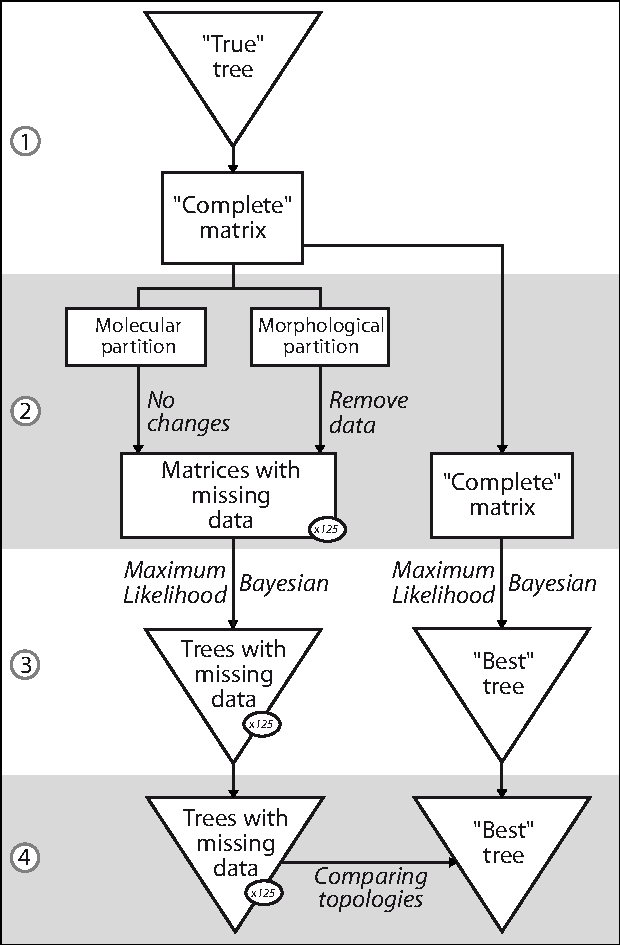
\includegraphics[keepaspectratio=true]{Figures/In_main/Simulations_outline-BW.pdf}
\caption{Protocol outline.
(1) We randomly generated a birth-death tree (the "true" tree) and used it to infer a matrix with no missing data (the "complete" matrix).
(2) We removed data from the morphological part of the "complete" matrix resulting in 125 "missing-data" matrices.
(3) We built phylogenetic trees from each matrix using both Maximum Likelihood and Bayesian methods.
(4) We compared the "missing-data" trees to the "best" tree.
We repeated these four steps 50 times.}
\label{Fig_Outline}
\end{figure}

%---------------------------------------------
%       1-Generating the matrix
%---------------------------------------------

\subsection{1. Generating the matrix}
\label{Generating_the_matrix}
First we randomly generated a "true" tree of 50 taxa in R v. 3.0.2 \citep{R302} using the package diversitree v. 0.9-6 \citep{fitzjohndiversitree2012}. We generated the tree using a birth death process by sampling speciation ($\lambda$) and extinction ($\mu$) rates from a uniform distribution but maintaining $\lambda$ $>$ $\mu$ \citep{paradistime-dependent2011}. We implemented a rejection sampling algorithm to select only trees with 25 living and 25 fossil taxa to ensure that we had enough taxa of each type for our missing data simulations to work. We then added an outgroup to the tree, using the mean branch length of the tree to separate the outgroup from the rest of the taxa, and with the branch length leading to the outgroup set as the sum of the mean branch length and the longest root-to-tip length of the tree.

Next, we generated a molecular and a morphological matrix from the "true" tree. The molecular matrix was inferred from the "true" tree using the R package phyclust v. 0.1-14 \citep{chen2011}. The matrix contained 1000 character sites for 51 taxa and was generated using the seqgen algorithm \citep{ranbaut1997seqgen} and using the HKY model \citep{HKY85} with random base frequencies and transition/transversion rate of two \citep{douadycomparison2003}. The substitution rates were distributed following a gamma distribution with an alpha ($\alpha$) shape of 0.5 \citep{yangamong-site1996}. We chose a low value of $\alpha$ to reduce the number of sites with high substitution rates, thus avoiding too much homoplasy and a decrease in phylogenetic signal. We selected the parameters above to generate data with no special assumption about how the characters evolved, and to reduce the computational time required if these parameters were estimated rather than defined in the tree building part of the analysis (even with the parameters defined, total computational time for the whole analysis was around 150 CPU years). All the molecular information for fossil taxa was replaced by missing data ("?").

We inferred the morphological matrix using the R package ape v. 3.0-11 \citep{paradisape:2004} to generate a matrix of 100 character sites for 51 taxa. We assigned the number of character states (either two or three) for each morphological character by sampling with a probability of 0.85 for two states characters and 0.15 for three state characters. These probabilities were selected using the overall distribution of character states extracted from 100 published empirical morphological matrices (see \hyperref[SupplementaryMaterial]{Supplementary Material Section 1}). We then ran an independent discrete character simulation for each character using the "true" tree with the character's randomly selected number of states (two or three) and assuming an equal rate of change (i.e. evolutionary rate) from one character state to another \citep{Pagel22011994}. This method allows us to have only two parameters for each character: the number of states and the evolutionary rate. For each character, the evolutionary rate was sampled from a gamma distribution with $\alpha$ = 0.5. We used low evolutionary rate parameters to avoid homoplasy in the morphological part of the matrix and create a clear phylogenetic signal \citep{wagner2000,davalosintegrating2014,wrightbayesian2014}.

Finally, we combined the morphological and molecular matrices obtained from the "true" tree. Hereafter we call this the "complete" matrix, i.e. the matrix with no missing data except for the molecular data of the fossil taxa.

%---------------------------------------------
%       2-Removing data
%---------------------------------------------

\subsection{2. Removing data}
\label{Removing_data}
We modified the "complete" matrix to get matrices with missing data by randomly replacing data with "?" in the morphological part of the matrices according to the following parameters:

\begin{enumerate}
\item{$M_{L}$, the proportion of living taxa with no morphological data: 0\%, 10\%, 25\%, 50\% or 75\%.}
This parameter illustrates the number of living taxa that are present in the molecular part of the matrix but not in the morphological part. This reflects the fact that detailed morphological data for living species are scarce.
\item{$M_{F}$, the proportion of missing data in the fossil taxa: 0\%, 10\%, 25\%, 50\% or 75\%.}
This parameter illustrates the quality of the fossil record. 
\item{$M_{C}$, the proportion of missing morphological characters for both living and fossil taxa: 0\%, 10\%, 25\%, 50\% or 75\%. }
This parameter illustrates the number of available morphological characters for both living and fossil taxa.
\end{enumerate}

In practice, each parameter represents a different way of removing data from the matrix: $M_{L}$ removes rows from the living taxa's data; $M_{F}$ removes cells from the fossil taxa's data; and $M_{C}$ removes columns across both living and fossil taxa's data. Note that $M_{L}$ and $M_{F}$ differ not only because of the region of the matrix affected: for $M_{L}$ all the morphological data of a percentage of living taxa are removed, whereas for $M_{F}$ a percentage of the data are removed at random from across the whole of the morphological matrix for fossil taxa.

We created matrices using all parameter combinations resulting in 125 ($5^3$) matrices. Note that one of these combinations has no missing data so is equivalent to the "complete" matrix, thus we have one effectively complete matrix in our 125 "missing-data" matrices. Because some parameter combinations introduce a lot of missing data (e.g. $M_L$ = 75\%, $M_F$ = 75\% and $M_C$ = 75\%), some matrices contained fossil taxa without any data at all. When this occurred we repeated the random deletion of characters until each taxon had at least 5\% data across the whole morphological part of the matrix.

%---------------------------------------------
%       3-Building phylogenies
%---------------------------------------------

\subsection{3. Building phylogenies}
From the resulting matrices we generated two types of trees: the "best" tree inferred from the "complete" matrix and the "missing-data" trees inferred from the 125 matrices with various amounts of missing data. The "true" tree was used to generate the "complete" matrix and reflects the "true" evolutionary history in our simulations. The "best" tree, on the other hand, is the best tree we can build using state-of-the-art phylogenetic methods. In real world situations, the "true" tree is never available to us because we cannot know the true evolutionary history of a clade (except in very rare circumstances, e.g. \citealt{rozen2005}). Therefore, here we focus on comparing the trees inferred from the matrices with missing data to the "best" tree, rather than the "true" tree, as the "best" tree is generally what we have to work with.

\subsubsection{Maximum Likelihood}
The "best" tree and the "missing-data" trees were inferred using RAxML v. 8.0.20 \citep{Stamatakis21012014}. For the molecular data, we used the GTR + $\Gamma_4$ model (\citealt{tavare1986}; default GTRGAMMA in RAxML v. 8.0.20; \citealt{Stamatakis21012014}). For the morphological data, we used the implemented Markov \textit{k} state model \citep{lewisa2001} assuming an equal state frequency and a unique overall substitution rate ($\mu$) following a gamma distribution of the rate variation with four distinct categories (M\textit{k} + $\Gamma_4$; -K MK option in RAxML v. 8.0.20; \citealt{Stamatakis21012014}).

To measure the phylogenetic signal of our simulations, we first ran a fast bootstrap analysis (Lazy Sub-tree Rearrangement) with 500 replicates on the "complete" matrix. We removed all the simulations with a median bootstrap support lower than 50 as a proxy for weak phylogenetic signal \citep{zanderminimal2004}. We repeated this selection until we obtained 50 sets of simulations (i.e. 50 "complete" and 50 x 125 "missing-data" matrices) with a relative good phylogenetic signal (median bootstrap $>$ 50). On these selected simulations, we used the fast bootstrap algorithm and performed 1000 bootstraps for each tree inference to assess topological support \citep{pattengale2010many}. Using these parameters took \texttildelow 8 CPU years to build 50 sets of 125 bootstrapped Maximum Likelihood trees (2.30GHz clock speed nodes).

\subsubsection{Bayesian}
The "best" tree and the "missing-data" trees were inferred using MrBayes v. 3.2.1 \citep{Ronquist2012mrbayes}. We partitioned the data to treat the molecular part as a non-codon DNA partition and the morphological part as a multi-state morphological partition. The molecular evolutionary history was inferred using the HKY model with a transition/transversion ratio of two \citep{douadycomparison2003} and a gamma distribution for the rate variation with four distinct categories (HKY + $\Gamma_4$). For the morphological data, we used the Markov \textit{k} state model \citep{lewisa2001}, with equal state frequency and a unique overall substitution rate ($\mu$) with four distinct rates categories (M\textit{k} + $\Gamma_4$). We chose these models to be consistent with the parameters used to generate the "complete" matrix.

Each Bayesian tree was estimated using two runs of four chains each for a maximum of 5$\times$$10^7$ generations. We used the following priors for each tree: (i) the "true" tree’s topology as a starting tree (with a starting value for each branch length of one), (ii) an exponential prior on the shape of the gamma distribution of $\alpha$ = 0.5 for both partitions, and (iii) a transition/transversion ratio prior of two sampled from a strong beta distribution ($\beta$(80,40)). We used these priors to speed up the Bayesian estimation process. These priors biased the way the Bayesian process calculated branch lengths by giving non-random starting points and boundaries for parameter estimation however, here we are focusing on the effect of missing data on tree topology and not branch lengths. Even using these priors, it took \texttildelow 140 CPU years to build 50 sets of 125 Bayesian trees (2.30GHz clock speed nodes). The detailed MrBayes parameters are available in the \hyperref[SupplementaryMaterial]{Supplementary Material S1}.

We used the average standard deviation of split frequencies (ASDS) as a proxy to estimate the convergence of the chains and used a stop rule when the ASDS went below 0.01 \citep{Ronquist2012mrbayes}. We also checked the effective sample size (ESS) on a random sub-sample of runs in each simulation to ensure that ESS $>>$ 200 \citep{drummond2006ess}. Finally we built a strict majority rule Bayesian consensus tree from the combined chains, excluding the 25\% first iterations as burn-in \citep{Ronquist2012mrbayes}.
%---------------------------------------------
%       4. Comparing Topologies
%---------------------------------------------

\subsection{4. Comparing topologies}
We compared the topology of the "missing-data" trees to the "best" tree to measure the effect of the three parameters $M_{L}$, $M_{F}$ and $M_{C}$ on tree topology. We used the Robinson-Foulds distance \citep{RF1981} to assess the amount of conserved clade positions and the Triplets distance \citep{dobson1975triplets} to assess the amount of wildcard taxa  (i.e. taxa that frequently change position in different trees; \citealt{kearneyfragmentary2002}). We normalised both metrics using methods described in \citet{Bogdanowicz2012} to generalize our results for any \textit{n} number of taxa. These metrics are described in detail below.

\subsubsection{Robinson-Foulds distance}
The Robinson-Foulds distance \citep{RF1981}, or "path difference", measures the number of shared clades across two trees. The metric reflects the distance between the distributions of tips among clades in the two trees (\citealt{RF1981}; see \hyperref[SupplementaryMaterial]{Supplementary Material S2} for calculation details). This metric is bounded between one, when the two trees are identical, and $n-2$ (for two trees with $n$ taxa) when there is no shared clade in the two trees. This metric is sensitive to minor changes in clade conservation: if the trees are composed of two clades of three taxa (\textit{(((a,b),c),((d,e),f))}), the swapping of any two taxa will lead to a maximal score of the Robinson-Foulds distance indicating poor tree similarity. We normalised this metric by dividing the Robinson-Foulds distance by the mean Robinson-Foulds distance from 1000 random tree comparisons \citep{Bogdanowicz2012}. This allows us to compare the metric for any number of taxa by scaling it with the expected value of the metric when comparing two random trees (see \hyperref[SupplementaryMaterial]{Supplementary Material S2} for the calculation details). Therefore, when the Normalised Robinson-Foulds distance between two trees is equal to one, the trees are identical; if the distance is equal to zero, the trees are no more different than expected by chance; finally if the distance is less than zero, the trees are more different than expected by chance.

\subsubsection{Triplets distance}
The Triplets distance \citep{dobson1975triplets} measures the number of sub-trees made up of three taxa that differ between two trees (\citealt{critchlowthe1996}; see \hyperref[SupplementaryMaterial]{Supplementary Material S2} for calculation details). This metric measures the position of each taxon and clade in relation to its closest neighbours. It is bounded between zero when the two trees are identical and $\binom{n}{4}$ (for two trees with $n$ taxa) when there is no shared taxa/clade position in the two trees. Therefore this metric sensitive to the conservation of wildcard taxa. We normalised this metric in the same way as for the Robinson-Foulds distance resulting in the Normalised Triplets distance.

\subsubsection{Paired tree comparisons}
\label{tree_comparisons}
For the Maximum Likelihood and Bayesian consensus trees we performed pairwise comparisons between the "best" tree and each "missing-data" tree using both the Normalised Robinson-Foulds and Normalised Triplets metrics with the TreeCmp java script \citep{Bogdanowicz2012} resulting in 125 Normalised Robison-Foulds distances and 125 Normalised Triplets distance for each tree inference method. Also, to take into account the uncertainty of tree inference, we extracted 1000 random bootstrapped trees from the Maximum Likelihood analysis and 1000 trees from the posterior tree distribution of the Bayesian analysis for the "best" trees, and then did the same for the 125 "missing data" trees (resulting in 1000 "best" trees and 125$\times$1000 "missing data" trees). 
For a given set of 1000 "missing data" trees and the 1000 "best" trees, we sampled one "missing data" tree and one "best" tree at random and compared them using both the Normalised Robinson-Foulds and Normalised Triplets metrics as described above. We repeated this 1000 times for each set of "missing data" trees resulting in 125$\times$1000 values for each metric. We repeated all the paired tree comparisons described above for each of the 50 simulation runs. We then calculated the mode and the 50\% and 95\% confidence intervals from the resulting distribution using the hdrcde R package v. 3.1 \citep{hdrcde}.

\subsection{Testing the effects of the missing data parameters on topological recovery}
Finally, we tested the effects of our missing data parameters ($M_{L}$, $M_{F}$, $M_{C}$ and their interactions) on our ability to recover the "best" tree topology in a Total Evidence framework. We also assessed the effect of our missing data parameters jointly with the effects of different tree inference and uncertainty methods (i.e. Maximum Likelihood, Bayesian consensus, Maximum Likelihood bootstrap trees and Bayesian posterior tree distribution).

We measured similarities among the distributions of the different metrics scores (Normalised Robinson-Foulds and Normalised Triplets distance) using the Bhattacharyya Coefficient \citep{Bhattacharyya}. The Bhattacharyya Coefficient is the probability of overlap between two distributions (\citealt{Bhattacharyya}; see \hyperref[SupplementaryMaterial]{Supplementary Material Section 2} for calculation details). Note that this is  equivalent to performing a two-sided t-test, but we use the Bhattacharyya Coefficient here because we are comparing distributions not means. To assess the effect of our missing data parameters, we calculated the Bhattacharyya Coefficient between the distributions of the different metrics scores (Normalised Robinson-Foulds and Normalised Triplets distance) for each pairwise combination of missing data parameters ($M_{L}$, $M_{F}$, $M_{C}$) and parameter states (0\%, 10\%, 25\%, 50\%, 75\%), i.e. $M_{L}$ = 0\%, $M_{F}$ = 0\%, $M_{C}$ = 0\%; $M_{L}$ = 10\%, $M_{F}$ = 0\%, $M_{C}$ = 0\% etc. (see Fig.~\ref{Fig_Bhattacharyya_Coefficients} for more details). This resulted in 7875 pairwise comparisons (a triangular matrix with $3^5$$\times$$3^5$ cells). We performed this procedure separately for each tree inference and uncertainty method. When two combinations of missing data parameters have a similar ability to recover the "best" tree topology the Bhattacharyya Coefficient will be close to one. Conversely, if the two combinations of missing data parameters differ, the Bhattacharyya Coefficient will be close to zero.

To assess the effect of the different tree inference and uncertainty methods (i.e. Maximum Likelihood, Bayesian consensus, Maximum Likelihood bootstrap trees and Bayesian posterior tree distribution) on our ability to recover the "best" tree topology, we calculated the Bhattacharyya Coefficient between the distributions of the different metrics scores (Normalised Robinson-Foulds and Normalised Triplets distance) for each pairwise combination of tree inference and uncertainty methods, i.e. Maximum Likelihood \textit{versus} Bayesian consensus; Maximum Likelihood \textit{versus} Maximum Likelihood bootstrap trees etc. (see Fig.~\ref{Fig_Bhattacharyya_Coefficients} for more details). Note that this procedure pools results from across all missing data parameter combinations so it results in just six pairwise comparisons. When two tree inference or uncertainty methods have a similar ability to recover the "best" tree topology the Bhattacharyya Coefficient will be close to one. Conversely, if the two tree inference or uncertainty methods differ, the Bhattacharyya Coefficient will be close to zero.

\begin{figure} 
\centering
    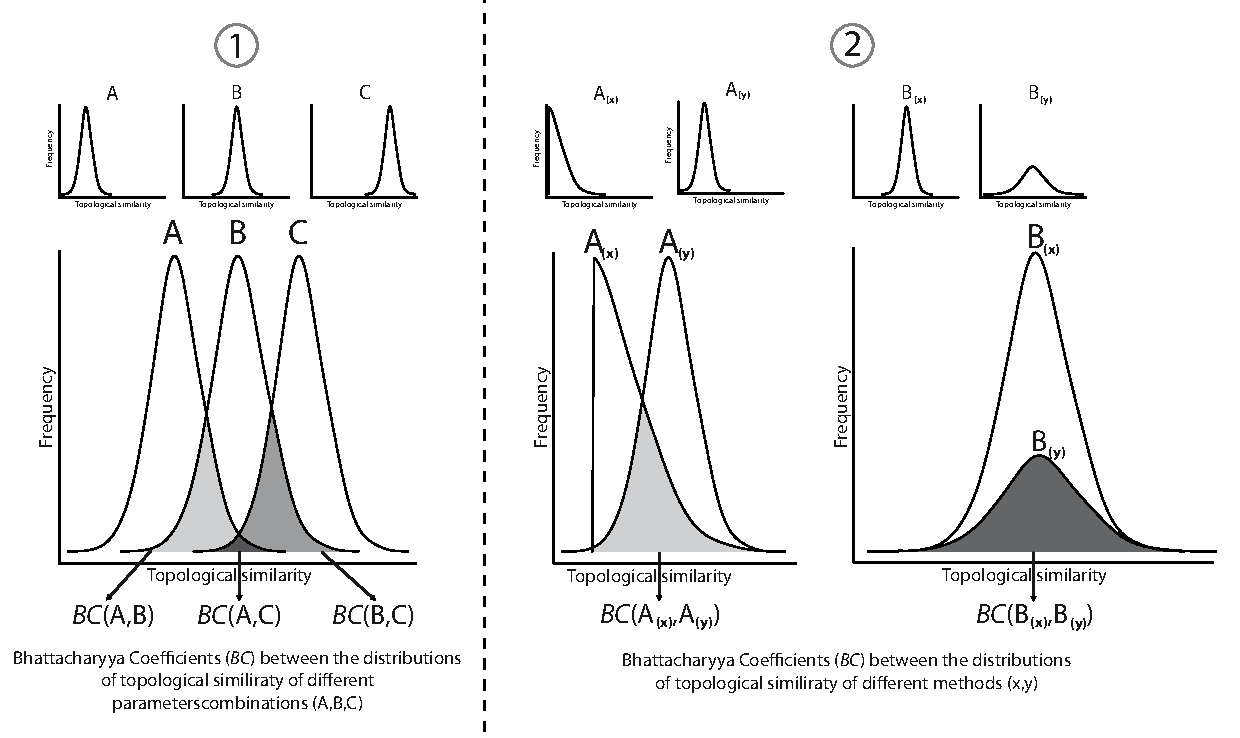
\includegraphics[width=1\textwidth]{Figures/In_main/Bhattacharyya_Coefficients.pdf}
\caption{Bhattacharyya Coefficient calculation outline. A, B and C are distribution of tree similarity (Normalised Robinson-Foulds or Normalised Triplets distances) for any combination of missing data parameters (e.g. $M_{L}$ = 10\%, $M_{F}$ = 50\%, $M_{C}$ = 75\%). \textbf{(x)} and \textbf{(y)} are two different tree inference methods (e.g. Maximum Likelihood or Bayesian). 1: the Bhattacharyya Coefficient (BC) is the overlap of the distribution of tree similarity between two combination of missing data parameters. 2: the Bhattacharyya Coefficient (BC) is the overlap of the distribution of tree similarity between two methods for the same combination of missing data parameters.}
\label{Fig_Bhattacharyya_Coefficients} %Bhattacharyya coefficients calculation outline
\end{figure}

%---------------------------------------------
%
%       RESULTS
%
%---------------------------------------------

\section{Results}
As the amount of missing data in the morphological part of the Total Evidence matrix increases, our ability to recover the "best" tree topology decreases, regardless of the missing data parameter ($M_{L}$, $M_{F}$ or $M_{C}$), the tree inference method (Maximum Likelihood or Bayesian) or the tree comparison metric used (Normalised Robinson-Foulds or Normalised Triplets distance). However, the different missing data parameters and tree inference methods do not affect the topology in the same way (Fig.~\ref{Fig_Results-permeth_perparam} and Fig.~\ref{Fig_Results-global_perparam}).

\begin{figure} 
\centering
    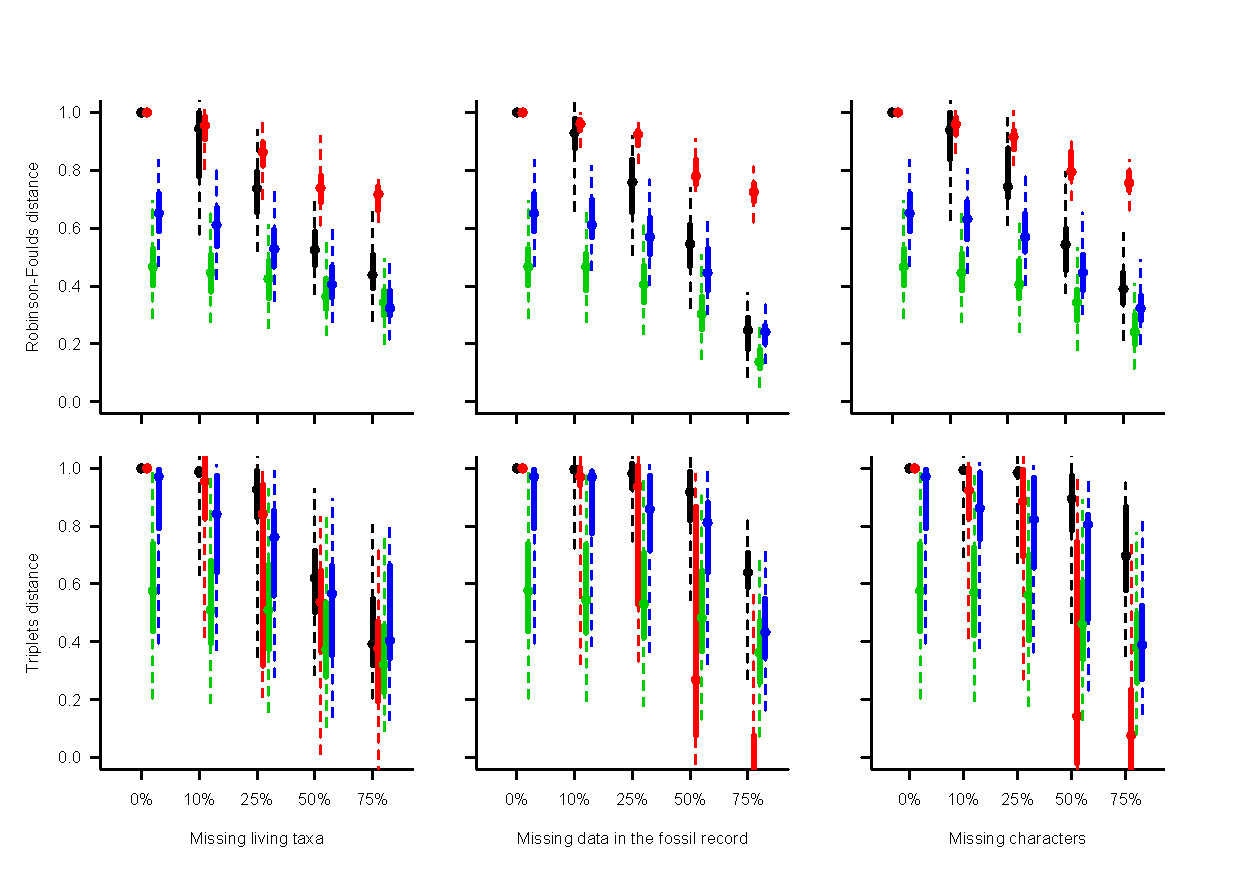
\includegraphics[width=1\textwidth]{Figures/In_main/AllMethods-RF+Tr-colour.pdf}
\caption{The effects of increasing missing data on topological recovery using Maximum Likelihood trees (black), Bayesian consensus trees (blue), Maximum Likelihood bootstrap trees (orange) and Bayesian posterior tree distributions (blue). The percentage of missing data for each parameter ($M_{L}$, $M_{F}$ and $M_{C}$) is shown on the x axis. Topological recovery was measured using two different tree comparison metrics: Normalised Robinson-Foulds distance (upper row) and Normalised Triplets distance (lower row). The graph shows the modal value (points), and the 50\% (thick solid lines) and 95\% (thin dashed lines) confidence intervals of the distributions of the tree comparison metric for each missing data parameter and tree inference method.}
\label{Fig_Results-permeth_perparam} %Differences within a subset of parameters and between methods
\end{figure}

\begin{figure} 
\centering
    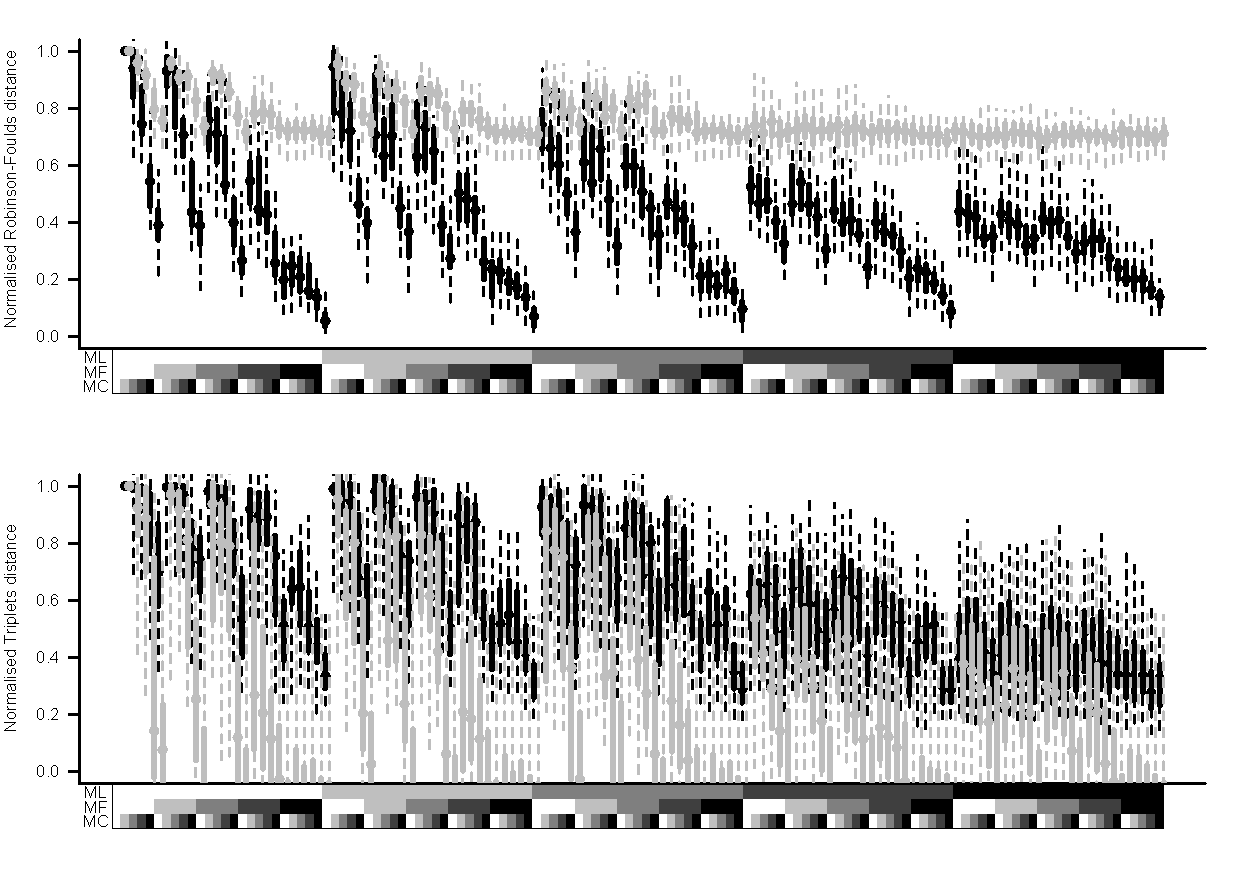
\includegraphics[width=1\textwidth]{Figures/In_main/ML+Baycon-AllParam-RF+Tr-BW.pdf}
\caption{The effects of increasing missing data on topological recovery using Maximum Likelihood trees (black) and Bayesian consensus trees (grey). The x axis shows the percentage of missing data from 0\% (white) to 75\% (black) for the three parameters: $M_{L}$ (upper line), $M_{F}$ (middle line) and $M_{C}$ (lower line). Topological recovery was measured using two different tree comparison metrics: Normalised Robinson-Foulds distance (upper row) and Normalised Triplets distance (lower row). The graph shows the modal value (points), and the 50\% (thick solid lines) and 95\% (thin dashed lines) confidence intervals of the distributions of the tree comparison metric for each missing data parameter and tree inference method.} 
\label{Fig_Results-global_perparam} %Differences between all the parameters and between two methods (ML vs BC)
\end{figure}

\subsection{Individual effects of missing data parameters}
As the amount of missing data increases across all three parameters, our ability to recover the "best" tree topology decreases (Fig.~\ref{Fig_Results-permeth_perparam}).
The Normalised Robinson-Foulds distance is always lower for the Maximum Likelihood trees than for the Bayesian consensus trees (median Bhattacharrya Coefficient = 0.69, 0.48 and 0.66 for $M_{L}$, $M_{F}$ and $M_{C}$ respectively; Fig.~\ref{Fig_Results-permeth_perparam}; \hyperref[SupplementaryMaterial]{Supplementary Material Section 3}: Tables S2-S4).
However, The Normalised Triplets distance is similar between the Maximum Likelihood trees and the Bayesian consensus trees for all the parameters ($M_{L}$, $M_{F}$ and $M_{C}$) (median Bhattacharrya Coefficient = 0.84, 0.75 and 0.80 for $M_{L}$, $M_{F}$ and $M_{C}$ respectively; Fig.~\ref{Fig_Results-permeth_perparam}; \hyperref[SupplementaryMaterial]{Supplementary Material Section 3}: Tables S2-S4).

\subsection{Combined effect of missing data parameters}
As expected, our ability to recover the "best" tree topology is worst when each parameter contains the maximum amount of missing data (i.e. $M_{L}$ = 75\%, $M_{F}$ = 75\% and $M_{C}$ = 75\%), and best when there is no missing data (i.e. $M_{L}$ = 0\%, $M_{F}$ = 0\%, $M_{C}$ = 0\%; Fig.~\ref{Fig_Results-global_perparam}; \hyperref[SupplementaryMaterial]{Supplementary Material Section 3}). Fig. ~\ref{Fig_Results-paircomp_within} shows the similarity of distributions of tree metrics in a triangular matrix with the values of each pairwise Bhattacharyya Coefficient coloured according to their values (orange when the distributions overlap completely, Bhattacharyya Coefficient = 1, and blue when they do not, Bhattacharyya Coefficient = 0; Fig.~\ref{Fig_Results-paircomp_within}). 

\begin{figure} 
\centering
     %Hide this figure for 'fast' build
%    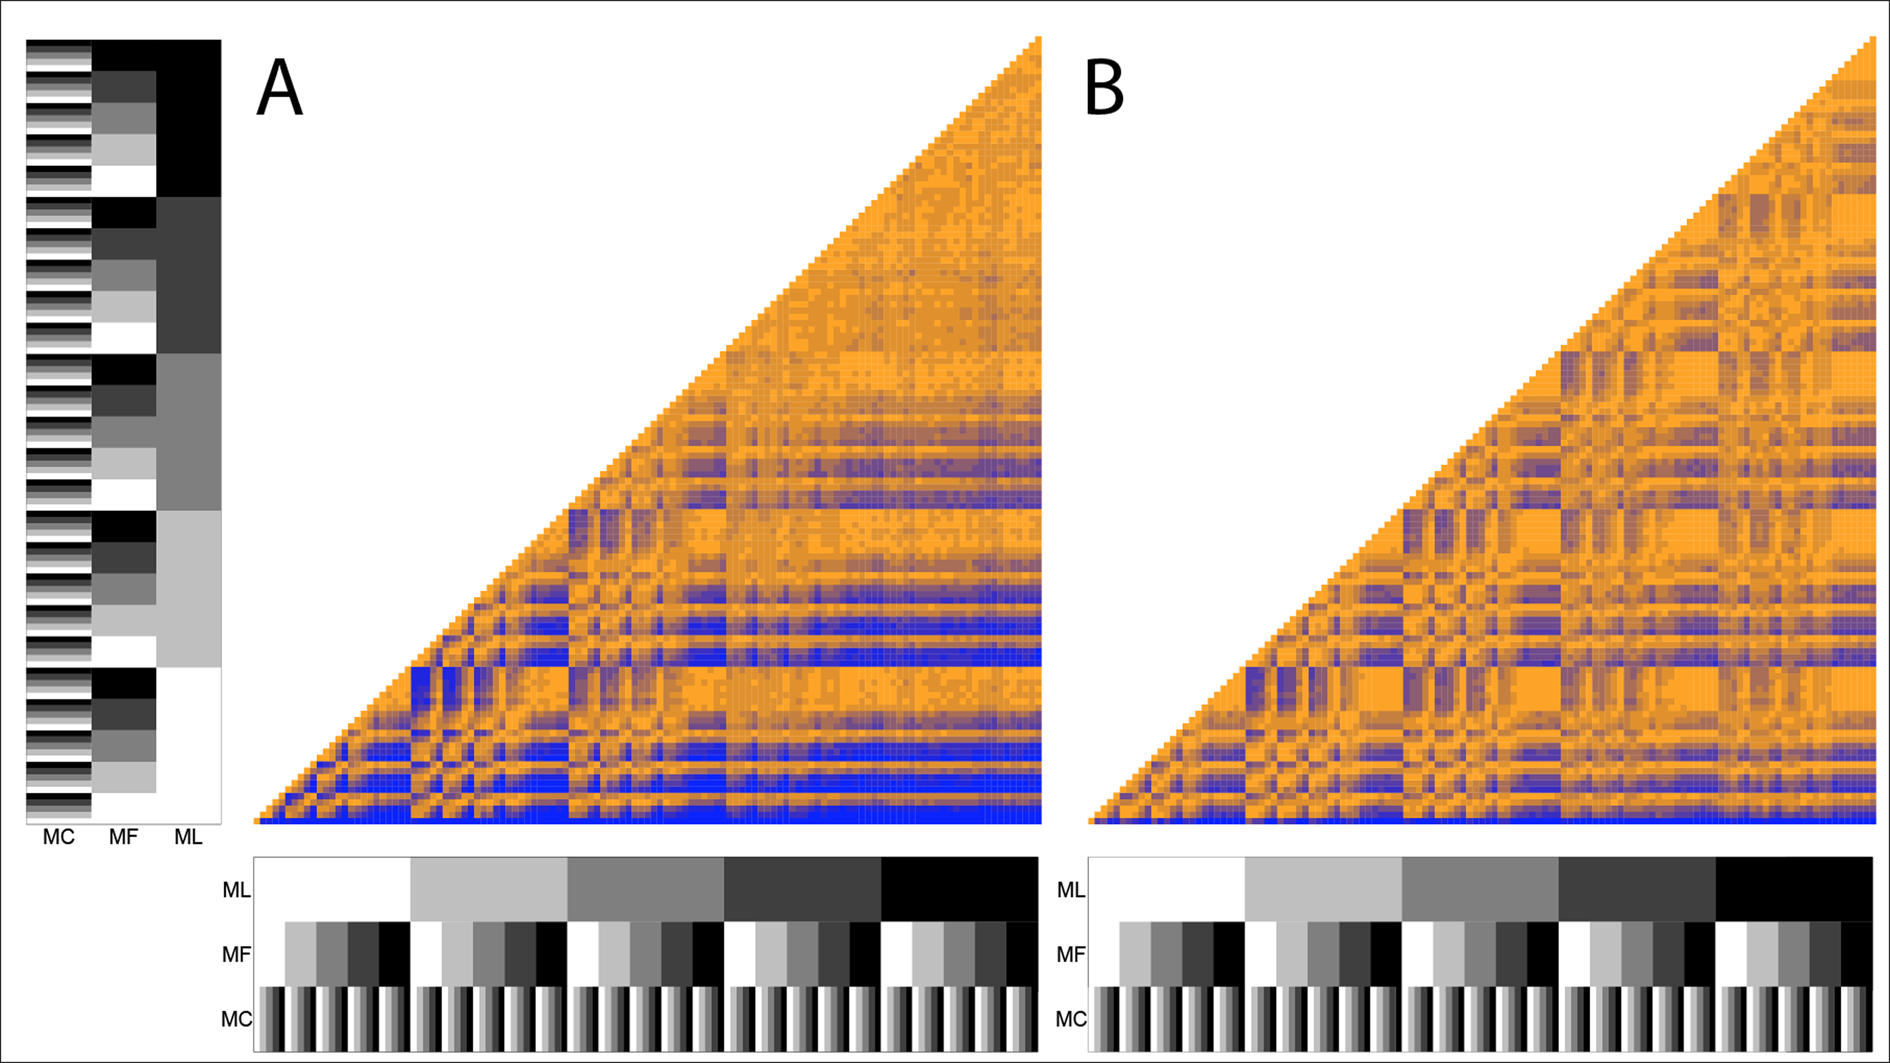
\includegraphics[width=1\textwidth]{Figures/In_main/PairwiseComp-Baycon-RF+Tr-colour.pdf}
    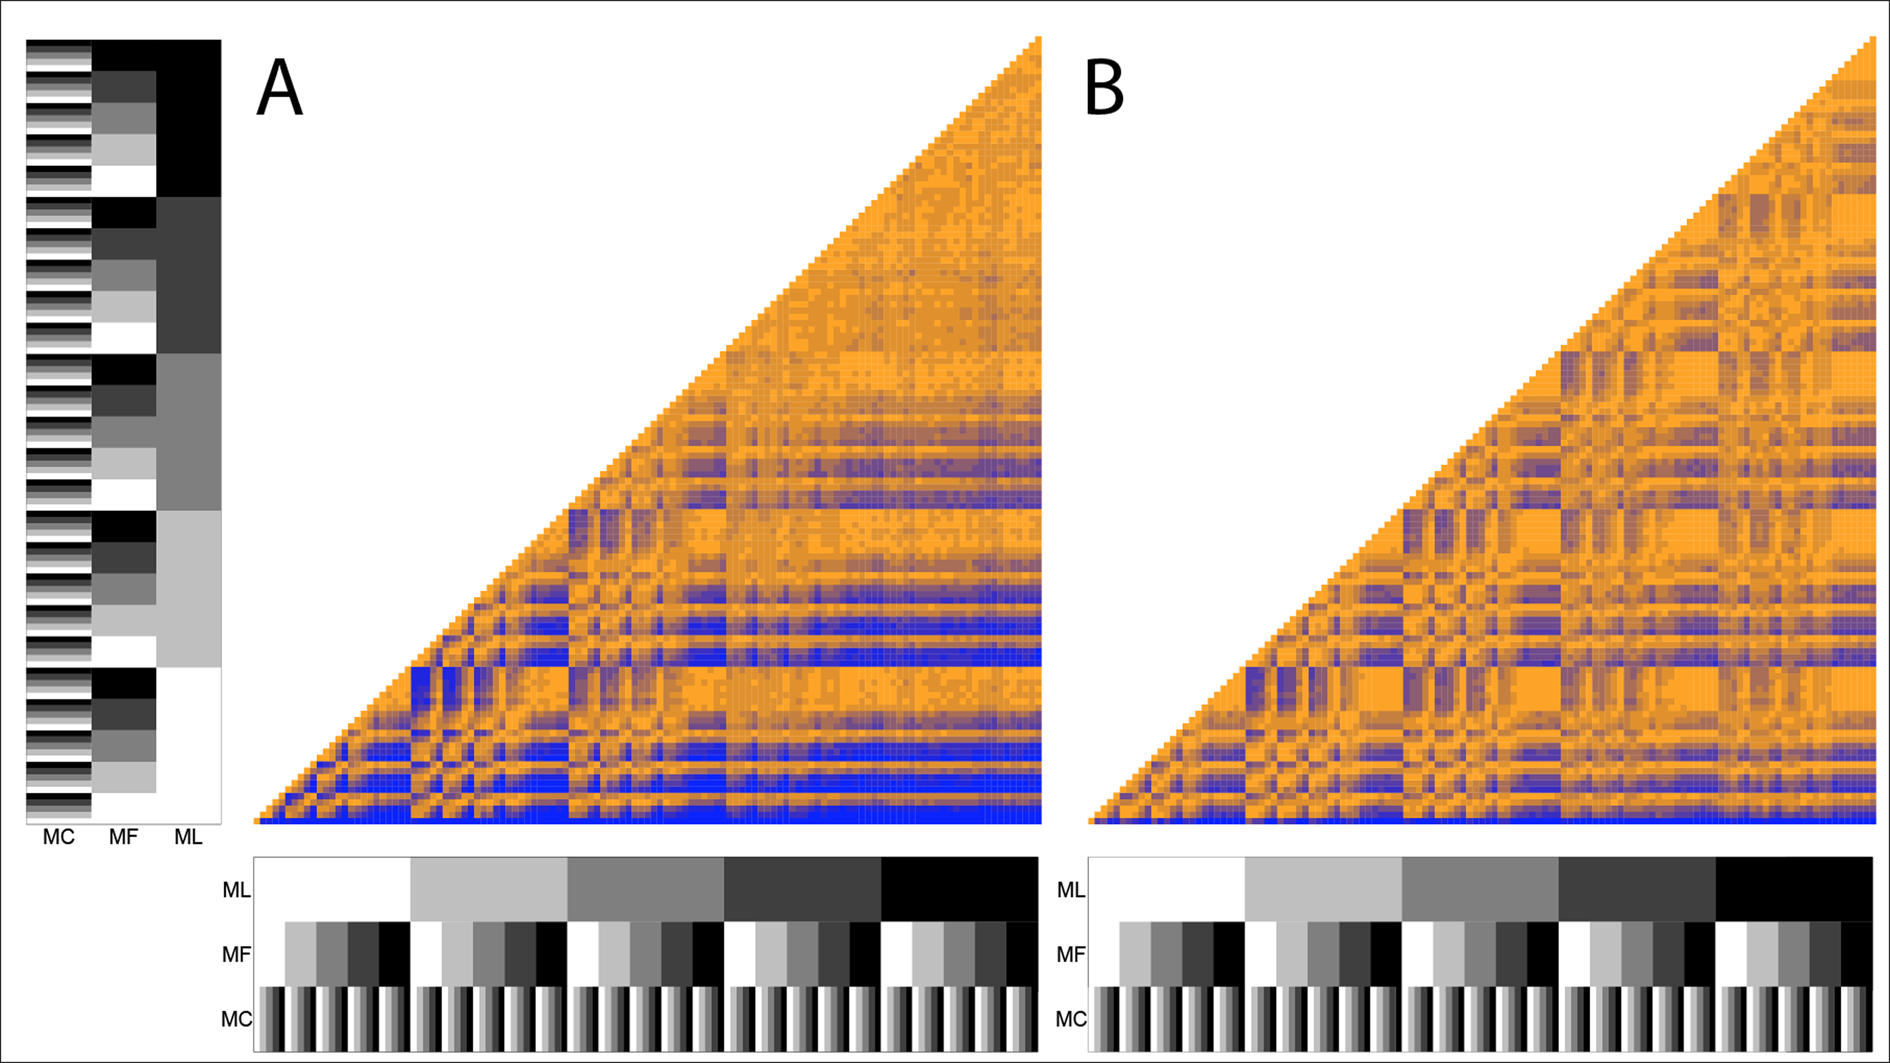
\includegraphics[width=1\textwidth]{Figures/In_main/PairwiseComp-Baycon-RF+Tr-colour.png} %bitmap version - 300 dpi RGB
\caption{The effects of missing data on topological recovery using Bayesian consensus trees. Both axes show the percentage of missing data from 0\% (white) to 75\% (black) for the three parameters: $M_{L}$ (upper line), $M_{F}$ (middle line) and $M_{C}$ (lower line). Topological recovery is represented by the probability of (A) Normalised Robinson-Foulds distance and (B) Normalised Triplets distance distributions overlapping with the "best" tree distribution, calculated using the Bhattacharyya Coefficient. The Bhattacharyya Coefficient values indicating low probability of overlap are shown in blue, those indicating a high probability of overlap are shown in orange.}
\label{Fig_Results-paircomp_within}
\end{figure} %Pairwise BC for the Bayesian consensus trees for RF and TR. (parameters differences)


Using both Normalised Robinson-Foulds and Normalised Triplets distances from the Bayesian consensus trees, the parameter combination with no missing data (i.e. $M_{L}$ = 0\%, $M_{F}$ = 0\%, $M_{C}$ = 0\%) is always the most dissimilar to all the other parameter combinations (Fig.~\ref{Fig_Results-paircomp_within}). However, the Normalised Robinson-Foulds distance (median Bhattacharrya coefficient = 0.79; Fig.~\ref{Fig_Results-paircomp_within}A) displays more dissimilarities than the Normalised Triplets distance (median Bhattacharrya coefficient = 0.81; Fig.~\ref{Fig_Results-paircomp_within}B). Additionally, when using the Normalised Robinson-Foulds distance, once $M_{L}$ $\geq$  50\%, there is no additional affect of $M_{F}$ and $M_{C}$, regardless of the amount of missing data in these parameters (Fig.~\ref{Fig_Results-paircomp_within}A). Likewise, once $M_{C}$ $\geq$ 50\%, there is no additional affect of $M_{L}$ and $M_{F}$ (Fig.~\ref{Fig_Results-paircomp_within}A).

For all combinations of missing data parameters and tree comparison metrics, the Maximum Likelihood bootstrap trees and the Bayesian posterior tree distributions perform very similarly (median Bhattacharrya Coefficient = 0.85 and 0.98, using Normalised Robinson-Foulds distance or Normalised Triplets distance respectively; Table ~\ref{Tab_Results-Difference_methods}). However, these two methods perform worse than the Bayesian consensus trees using Normalised Robinson-Foulds distance (median Bhattacharrya Coefficient = 0 and 0.01, for the Maximum Likelihood bootstrap trees and the Bayesian posterior tree distribution respectively; Table ~\ref{Tab_Results-Difference_methods}; Fig.~\ref{Fig_Results-permeth_perparam} and \hyperref[SupplementaryMaterial]{Supplementary Material Section 3}).

% NC: In the caption you need to explain why some of these values are in bold...
\begin{landscape}
\begin{table}[ht]
\caption{Bhattacharyya Coefficients of the pairwise method comparisons, each of which corresponds to the normalised distance between the "best" tree and the "missing data" using either the Normalised Robinson-Foulds distance (RF) or the Normalised Triplets distance (Tr). The values in bold are the extreme values of high or low probability of overlap between two methods.}
\centering
\begin{tabular}{lccccccc}
  \hline
 Comparison &  Metric & Min. & 1st Qu. & Median & Mean & 3rd Qu. & Max. \\ 
  \hline
    Maximum Likelihood \textit{vs.} Bayesian consensus                 & $RF$ & 0.00 & 0.00 & 0.10 & 0.20 & 0.32 & 1.00 \\ 
                                                                       & $Tr$ & 0.34 & 0.49 & 0.61 & 0.62 & 0.75 & 1.00 \\ 
    Maximum Likelihood \textit{vs.} Maximum Likelihood bootstraps      & $RF$ & 0.03 & 0.54 & 0.69 & 0.64 & 0.77 & 0.98 \\ 
                                                                       & $Tr$ & 0.08 & 0.57 & 0.65 & 0.64 & 0.73 & 0.82 \\ 
    Maximum Likelihood \textit{vs.} Bayesian posterior trees           & $RF$ & 0.02 & 0.74 & 0.80 & 0.79 & 0.89 & 0.98 \\ 
                                                                       & $Tr$ & 0.21 & 0.67 & 0.73 & 0.72 & 0.77 & 0.84 \\ 
    Bayesian consensus \textit{vs.} Maximum Likelihood bootstraps      & $RF$ & 0.00 & 0.00 & \textbf{0.00} & \textbf{0.01} & 0.01 & 0.04 \\ 
                                                                       & $Tr$ & 0.08 & 0.38 & 0.59 & 0.57 & 0.73 & 0.84 \\ 
    Bayesian consensus \textit{vs.} Bayesian posterior trees           & $RF$ & 0.00 & 0.00 & \textbf{0.01} & \textbf{0.02} & 0.04 & 0.11 \\ 
                                                                       & $Tr$ & 0.21 & 0.36 & 0.56 & 0.55 & 0.74 & 0.87 \\ 
    Bayesian posterior tree \textit{vs.} Maximum Likelihood bootstraps & $RF$ & 0.50 & 0.77 & \textbf{0.85} & \textbf{0.85} & 0.96 & 1.00 \\ 
                                                                       & $Tr$ & 0.91 & 0.96 & \textbf{0.98} & \textbf{0.97} & 0.99 & 1.00 \\ 
   \hline
\end{tabular}
\label{Tab_Results-Difference_methods}
\end{table}
\end{landscape}

%---------------------------------------------
%
%       DISCUSSION
%
%---------------------------------------------

\section{Discussion}

Our results show that the ability to recover the "best" tree topology in a Total Evidence framework decreases as the amount of missing data increases, regardless of how data were removed or the method of tree inference used. However, these factors affected topological recovery in different ways and to different extents. 
Decreasing the amount of living taxa with morphological data ($M_{L}$) and the overall number of morphological characters in the matrix ($M_{C}$) had worst effects on topological recovery (Fig.~\ref{Fig_Results-paircomp_within}). Additionally, using Bayesian consensus trees recovered the "best" tree topology more consistently than using Maximum Likelihood trees or Bayesian posterior tree distributions (Fig.~\ref{Fig_Results-global_perparam}, Fig.~\ref{Fig_Results-paircomp_within}, Table 1). As seen in previous studies, our results show that the amount of missing data is not a problem \textit{per se} for Total Evidence methods, as long as enough living and fossil taxa in the matrix have data for overlapping morphological characters \citep[e.g.][]{kearneyfragmentary2002,wiensmissing2003,rouresite-specific2011,pattinsonphylogeny2014}. 

\subsection{Individual effects of missing data parameters}
\subsubsection{Missing data for living taxa ($M_{L}$)}
When the number of living taxa with morphological data ($M_{L}$) decreases, entire rows of data are being removed from the living taxa part of the matrix. Because living taxa still have molecular characters available for phylogenetic inference (see \hyperref[Generating_the_matrix]{methods}),even if they have no morphological data, the relationships among them will always be fairly well-resolved (depending on the phylogenetic signal from the molecular part of the matrix).  However, this missing data parameter has a huge influence on the placement of fossil taxa because a decrease in the $M_{L}$ parameter reduces the amount of overlapping data among the living and fossil taxa, meaning there is no part of the living taxa tree that the fossils can branch off.

\subsubsection{Missing data for fossil taxa ($M_{F}$)}
When the overall proportion of data for the fossil taxa ($M_{F}$) decreases, this also reduces the probability of morphological characters for fossil taxa overlapping with the ones for living taxa. This can lead to difficulties for the placement of certain taxa in the tree. However, it is important to note that even though the number of displaced wildcard taxa increases (i.e. decrease of Normalised Triplets distance) with increasing missing data in this parameter, clade conservation (i.e. Normalised Robinson-Foulds distance) is still relatively good (mode = 0.72) when the proportion of missing data is high ($M_{F}$ = 75\%).

The effect of the missing data in the fossil record ($M_{F}$) is less than the effect of the $M_{L}$ parameter on clade conservation (Normalised Robinson-Foulds distance) but greater on the displacement of wildcard taxa (Normalised Triplets distance; Fig.~\ref{Fig_Results-permeth_perparam} and Fig.~\ref{Fig_Results-global_perparam}). This is related to the fact that the Bayesian consensus tree is built using a majority consensus rule. When the fossil taxa have less data (e.g. $M_{F}$ = 75\%) they will tend to branch with any taxon in the clade that shares most characters with the fossils. Therefore a majority consensus position is unlikely to exist (i.e. every branching position is represented in $<$ 50\% of the trees in the Bayesian posterior distribution) and the fossil taxa will form a polytomy at the base of the clade. This does not decrease the Normalised Robinson-Foulds distance, because clades are conserved, but decreases the Normalised Triplets distance because the fossils act as wildcard taxa. Conversely, the same scenario in a Maximum Likelihood framework will lead to a dichotomous branching of the fossils but with low bootstrap support ($<$ 50). In other words, the Bayesian consensus tree allows a fossil taxon with few data to be placed with a higher confidence at a lower taxonomic level than the Maximum Likelihood tree, where the fossil will be placed with lower confidence at a higher taxonomic level. We argue that using the Bayesian consensus tree topology is preferable because it is more conservative \cite[e.g][]{pattinsonphylogeny2014}.

\subsubsection{Missing morphological characters ($M_{C}$)}
Reducing the overall number of morphological characters reduces the probability of their overlap among the taxa in the matrix, and therefore decreases our ability to recover the "best" tree topology. We expected the decrease in this parameter to have an effect twice as large as that for the $M_{L}$ and $M_{F}$ parameters, because removing 10\% of the data for the fossil or living taxa only removes 5\% of data from the whole matrix (because this parameter affects only half of the taxa present in the matrix). Conversely, removing 10\% of morphological characters ($M_{C}$) genuinely removes 10\% of data in the matrix. However, the effect of removing characters on the ability to recover the "best" tree topology is of the same order of magnitude as for the other two parameters (Fig.~\ref{Fig_Results-permeth_perparam}). We suspect this again reflects the importance of overlapping characters, as opposed to the number of characters \textit{per se}.

Additionally, the number of morphological characters determines the size the matrix. This can affect our ability to recover the "best" tree topology through: (1) the incongruence of phylogenetic signal among morphological and molecular data; and/or (2) homoplasy. The incongruence of phylogenetic signal between morphological and molecular data has previously been demonstrated to be more important in small morphological matrices \citep{wagner2000}. The size of our data matrices were constrained by the performance of our protocol: to reduce the computational time of our analysis to a reasonable level (150 CPU years), we ran our simulations on modestly-sized matrices of 1000 molecular characters and 100 morphological characters. Therefore, part of the decrease of the Normalised Robinson-Fould distance and the Normalised Triplets distance in our simulations could be due to conflicting phylogenetic signal among morphological and molecular data in our matrices (Fig.~\ref{Fig_Results-permeth_perparam} and Fig.~\ref{Fig_Results-global_perparam}). However, although these matrices are an order of magnitude smaller than some published matrices \citep[e.g.][]{springermacroevolutionary2012,nithe2013}, they are still within the size range of more modestly-sized empirical matrices \citep[e.g.][]{kellymolecular2014, sallam2011craniodental}. Therefore, our simulations reflect realistic parameters. Homoplasy, on the other hand, is expected to increase with an increase in the number of morphological characters \citep{wrightbayesian2014}. % NC: Missing a citation here. Also is this correct - increase and increase? TG: yep. Checking for a better cite though.
However, the use of probabilistic methods (i.e. Maximum Likelihood or Bayesian) and the M\textit{k} model \citep{lewisa2001} has been previously demonstrated to partially resolve this issue \citep{wrightbayesian2014}.

\subsection{Combined effect of missing data parameters}
As expected, when combining the missing data parameters, our ability to recover the "best" tree topology is affected in the same way as for the parameters individually: the Normalised Robinson-Foulds distance and the Normalised Triplets distance are higher when all the missing data parameters have few missing data (i.e. $M_{L}$ = 0\%, $M_{F}$ = 0\%, $M_{C}$ = 0\%) and lower when they have a lot of missing data (i.e. $M_{L}$ = 75\%, $M_{F}$ = 75\% and $M_{C}$ = 75\%; Fig.~\ref{Fig_Results-global_perparam}). However, it is important to notice that the effect of each parameter is not additive. The number of missing living taxa with morphological data ($M_{L}$) and the overall number of missing morphological characters ($M_{C}$), have a bigger effect than the amount of missing data for the fossil taxa ($M_{F}$), and when both $M_{L}$ and $M_{C}$ reach 50\% of missing data, the matrix does not contain enough phylogenetic information for the fossil taxa to be placed with confidence in the tree (Fig.~\ref{Fig_Results-paircomp_within}). This has important implications for building Total Evidence phylogenies (see below).

\subsection{Effects of tree inference methods}
Variation in our ability to recover the "best" tree topology depends heavily on the tree inference method (Fig.~\ref{Fig_Results-permeth_perparam} and Fig.~\ref{Fig_Results-global_perparam}). For morphological data, previous studies have shown some superiority of probabilistic tree inference methods with simple evolutionary models such as the M\textit{k} model \citep{lewisa2001} over cladistic methods (\citealt{wrightbayesian2014}; but see \citealt{spencerefficacy2013}). However, this is the first study, to our knowledge, to compare the performance of the M\textit{k} model \citep{lewisa2001} for recovering the "best" tree topology using Maximum Likelihood and Bayesian methods in a Total Evidence framework. Our results show that the topology of the Bayesian consensus tree is always closer to the "best" tree topology than the one of the Maximum Likelihood tree (Fig.~\ref{Fig_Results-global_perparam}). As described above, this is because the Bayesian consensus tree allows a fossil taxon with few data to be placed with a higher confidence at a lower taxonomic level than the Maximum Likelihood tree. 

It is also worth noting that across all our analyses, the topologies of the Maximum Likelihood bootstrap trees and the Bayesian posterior trees distribution were always further from the "best" tree topology than Maximum Likelihood and Bayesian consensus trees. This was true even when no morphological data was missing ($M_{L}$ = 0\%; $M_{F}$ = 0\%, $M_{C}$ = 0\%; Fig.~\ref{Fig_Results-permeth_perparam}). This reflects the fact that it is difficult to compare two distributions of trees, and each comparison between a set of "missing data" trees and a set of the "best" trees involved 1000 random pairwise comparisons rather than just one. This will obviously add noise to the results for these methods.

\subsection{Practical implications}
Our missing data parameters illustrate different sources of missing data in empirical matrices as follows: ($M_{L}$) the paucity of coded morphological characters for living taxa; ($M_{F}$) the missing data for fossils (or parts of fossils) that have not been preserved in the fossil record; and ($M_{C}$) characters that have not been coded across living and fossil species, perhaps due to difficulties in coding or poor preservation of the feature in collections. Filling these gaps in empirical Total Evidence matrices should lead to a substantial increase in our ability to recover the "best" tree topology. We can increase the number of living taxa with coded morphological characters by increasing research efforts in this area, and encouraging use of our vast natural history collections. Increasing data for fossil species is harder, since it depends on fossil preservation biases and new fossil discoveries. However, gaps in the matrix can be filled with efforts in palaeontological field work that can potentially lead to future discoveries of exceptionally preserved fossils \citep[e.g.][]{nithe2013}. Fortunately, although this data is the most difficult to collect, it also has the least influence on whether our simulations recover the "best" tree topology (Fig.~\ref{Fig_Results-paircomp_within}). Finally, although increasing the number of coded characters is relatively straightforward, the amount of time it takes to build a morphological matrix increases directly with the number of characters involved. One solution to this problem may be to engage with collaborative data collection projects through web portals such as \textit{morphobank} \citep{morphobank}, so that no one individual collects all the data.

Another practical implication of our results regards the tree inference methods. Because the Bayesian consensus trees consistently recovered topologies closer to the "best" tree topology than the Maximum Likelihood trees, we advise using Bayesian consensus trees to fix the topology where necessary for further steps in tree inference, for example in Tip-Dating \citep{ronquista2012,BEASTmaster}. Note that, although the Bayesian posterior tree distribution performed poorly in recovering the "best" tree topology, this is due to difficulties comparing distributions of trees (see discussion above). Thus, we do not suggest discarding the Bayesian posterior tree distribution once the topology has been fixed, particularly because these trees will be invaluable for phylogenetic comparative analyses \citep[e.g.][]{jetzthe2012}.
    
%---------------------------------------------
%
%       CONCLUSION
%
%---------------------------------------------

\section{Conclusion}

Missing data in Total Evidence matrices is not a problem for recovering the "best" tree topology as long as enough living and fossil taxa in the matrix have data for overlapping morphological characters. When missing data increases in any of our missing data parameters ($M_{L}$, $M_{F}$ or $M_{C}$), it reduces support for the placement of fossil taxa and increases the displacement of wildcard taxa. Therefore we advise filling as many gaps in Total Evidence matrices as possible. Because this is difficult, if not impossible, for fossil data, we recommend coding as many morphological characters, for as many living taxa, as possible. Additionally, the topology of the Bayesian consensus trees, regardless the amount of missing data, were always closer to the "best" tree topology than the Maximum Likelihood trees. Therefore, we advise using Bayesian consensus tree topologies if topology must be fixed in a Total Evidence analysis, for example when using the Tip-Dating method. The results of our analyses are encouraging and show that it is possible to combine both neontological and palaeontological data in the same phylogeny despite issues of missing data. Hopefully, using these approaches will greatly improve our understanding of macroevolutionary processes through both time and space.

%---------------------------------------------
%
%       ...
%
%---------------------------------------------
\section{Supplementary material}
Supplementary material (R code, analyses, supplementary methods and full results) can be found in the Dryad data repository at http://dx.doi.org/10.5061/dryad.XXXX.

\section{Acknowledgments}
Thanks to Gavin Thomas, Fr\'{e}d\'{e}ric Delsuc, Emmanuel Douzery, Trevor Hodkinson, Andrew Jackson, and April Wright for useful comments on our simulation protocol. Thanks to Paddy Doyle, Graziano D'Innocenzo and Sean McGrath for assistance with the computer cluster. Simulations used the Lonsdale cluster maintained by the Trinity Centre for High Performance Computing and funded through grants from Science Foundation Ireland. This work was funded by a European Commission CORDIS Seventh Framework Programme (FP7) Marie Curie CIG grant (proposal number: 321696).

%cite cheat sheet
 % The \cite command functions as follows:
 %   \citet{key} ==>>                Jones et al. (1990)
 %   \citet*{key} ==>>               Jones, Baker, and Smith (1990)
 %   \citep{key} ==>>                (Jones et al., 1990)
 %   \citep*{key} ==>>               (Jones, Baker, and Smith, 1990)
 %   \citep[chap. 2]{key} ==>>       (Jones et al., 1990, chap. 2)
 %   \citep[e.g.][]{key} ==>>        (e.g. Jones et al., 1990)
 %   \citep[e.g.][p. 32]{key} ==>>   (e.g. Jones et al., p. 32)
 %   \citeauthor{key} ==>>           Jones et al.
 %   \citeauthor*{key} ==>>          Jones, Baker, and Smith
 %   \citeyear{key} ==>>             1990

\bibliographystyle{sysbio}
\bibliography{References}

%---------------------------------------------
%
%       Supplementary
%
%---------------------------------------------

%Ignore this for 'fast' pdf building
\newpage
\section{Supplementary Material}

    \documentclass[12pt,letterpaper]{article}

%Packages
\usepackage{pdflscape}
\usepackage{fixltx2e}
\usepackage{textcomp}
\usepackage{fullpage}
\usepackage{natbib}
\usepackage{float}
\usepackage{latexsym}
\usepackage{url}
\usepackage{epsfig}
\usepackage{graphicx}
\usepackage{amssymb}
\usepackage{amsmath}
\usepackage{bm}
\usepackage{array}
\usepackage[version=3]{mhchem}
\usepackage{ifthen}
\usepackage{caption}
\usepackage{hyperref}
\usepackage{amsthm}
\usepackage{amstext}
\usepackage{enumerate}
\usepackage[osf]{mathpazo}
\usepackage{dcolumn}
\usepackage{lineno}
\pagenumbering{arabic}


%Pagination style and stuff
\linespread{2}
\raggedright
\setlength{\parindent}{0.5in}
\setcounter{secnumdepth}{0} 
\renewcommand{\section}[1]{%
\bigskip
\begin{center}
\begin{Large}
\normalfont\scshape #1
\medskip
\end{Large}
\end{center}}
\renewcommand{\subsection}[1]{%
\bigskip
\begin{center}
\begin{large}
\normalfont\itshape #1
\end{large}
\end{center}}
\renewcommand{\subsubsection}[1]{%
\vspace{2ex}
\noindent
\textit{#1.}---}
\renewcommand{\tableofcontents}{}
\bibpunct{(}{)}{;}{a}{}{,}

\section{Code}
All code for performing the analyses is available at: \url{https://github.com/TGuillerme/Total_Evidence_Method-Missing_data}.

\newpage
\section{Appendix 1: Tree Building}
  \section{Supplementary material Section 1}

\subsection{Morphological characters states}
In order to obtain a realistic probabilistic value for of \textit{k} characters states for each simulated morphological character, we downloaded 100 random morphological characters (with more than 100 characters each) from TreeBASE database (http://treebase.org/) published between 1985 and 2013 and covering 19 taxomomic classess (Chordata, Arthropoda, Annelida, Angiosperm, Gymnosperm and Pteridophyta).
We selected a total of 22563 characters ranging from 2 to 10 states.
We calculated the proportion of characters with 2, 3, 4, 5, 6, 7, 8, 9 or 10 states.
We then sampeled 22563 \textit{k} values between 2 and 10 with the same proportion of characters from the empirical data.
We then used a simple t-test to check if our simulation was equal to the empirical data.
In this study, we only simulated characters with 2 or 3 states because of the high proportion of ordered characters ecountered on characters with more than 3 states and the difficulties of simulate biologicaly sensible ordered characters.

\begin{figure}
\centering
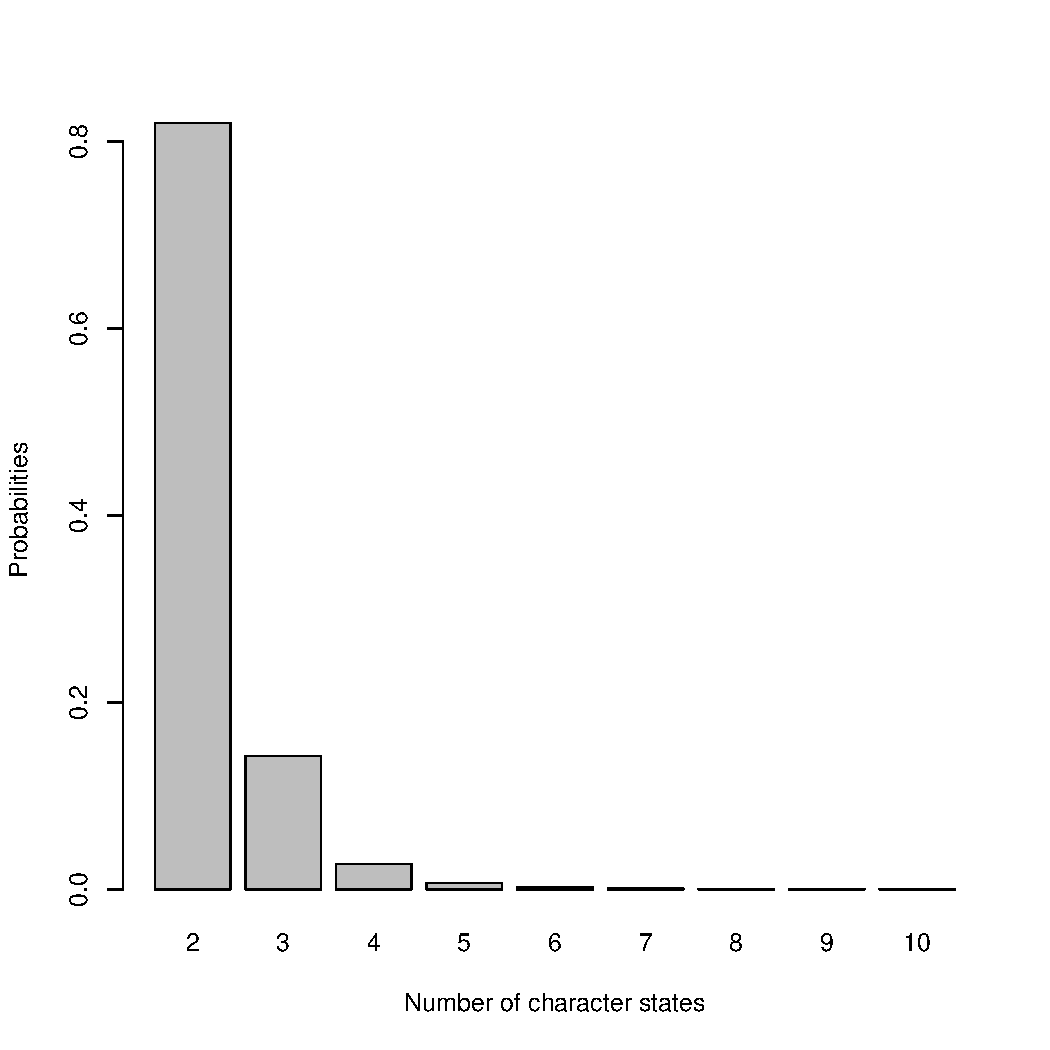
\includegraphics[keepaspectratio=true]{Figures/Supplementary/TEM_Fig-AppendixCharacters.pdf}
\caption{Character states distribution in empirical matrices. %Title?
Characters states number distribution extracted from 100 random morphological matrices downloaded from RreeBase.}
\label{Fig_AppendixCharacters}
\end{figure}


\subsection{Tree Building Software settings}

\subsubsection{Maximum Likelihood - RAxML v8.0.20 \citep{Stamatakis21012014}}

Model: \\
Molecular data: \\
GTR + $\Gamma_4$ (-m GTRGAMMA) \\
Morphological data: \\
Mk + $\Gamma_4$ (-K MK) \\
Support: \\
Rapid Boostrap algorithm (LSR), 1000 replicates \\

\subsubsection{Bayesian - MrBayes v3.2.1 \citep{Ronquist2012mrbayes}}

Priors: \\
Molecular data: \\
rates distribution shape ($\alpha$) = 0.5 \\
Transition/Transversion ratio = 2 ($\beta$(80,40)) \\
Starting tree: "True" tree topology with each branch length = 1 \\
Morphological data: \\
rates distribution shape ($\alpha$) = 0.5 \\
Models: \\
Molecular data: HKY + $\Gamma_4$ \\
Morphological data: Mk + $\Gamma_4$ \\
MCMC: \\
2 runs \\
4 chains per run \\
generations < 50$\times$$1^6$ \\
sample frequency = 1050$\times$$1^3$ \\
ASDS diagnosis frequency = 50$\times$$1^3$ \\
ASDS $<$ 0.01 \\
ESS $>>$ 200 \\
Burnin = 25\%
  \label{Supp_TreeBuilding}

\newpage
\section{Appendix 2: Tree Comparisons}
  %\section{Supplementary material Section 2}

\subsection{Robinson-Foulds distance}
Robinson-Foulds distance (\textit{RF}; \citealp{RF1981}), or "path difference", measures the number of shared clades across two trees. The metric reflects the distance between the distributions of tips among clades in the two trees \citep{RF1981} and can be expressed as:
\begin{equation}
RF_{x,y} = N_{x} + N_{y} - 2C_{x,y}
\end{equation}
where $C_{x,y}$ is the number of clades in common in the two trees. $C$ is equal to one if the two trees have the same $n$ taxa; and $C = n-2$ when none of the $n$ taxa are shared between the trees. This metric is more sensitive to taxon displacement than Triplets distance (i.e. if one taxon moves out of a clade, then the clades are no longer considered similar; \citet{critchlowthe1996,johnson1998,wiensmissing2003}). The minimal value of $C$ is equal to 1 if the two trees have the same n taxa; the maximal value in $C = n-2$. For a fully unresolved tree (star tree) $N$=1 and for a fully resolved tree (binary tree) $N = n-2$. The minimal and maximal topological distance for taxa is:
\begin{equation}
RF_{min} = 1 + 1 - 2C_{x,y}
\end{equation}
and:
\begin{equation}
RF_{max} = 2(n-2)-2
\end{equation}
One can then rescale \textit{RF.scaled} by using the maximal and minimal value for any $n$ taxa:
\begin{equation}
RF.scaled_{x,y} = \frac{RF_{x,y}-RF_{max}}{RF_{max}}
\end{equation}
This metric is more sensitive to taxa displacement than the Triplets distance \citep{critchlowthe1996,johnson1998,wiensmissing2003} and therefore a low value will show a good clade conservation between two trees and a high value will show a bad recovery of common clades.

\subsection{Triplets distance details ($T_{x,y}$)}
Triplets distance ($T_{x,y}$; \citealp{dobson1975triplets}) measures the number of sub-trees made up of three taxa (triplets) that differ between two given trees. Each triplet can be written as $I_{ijk}$=(\textit{ijk}). Where $I_{ijk}$ is equal to zero if the the two triplets (\textit{ijk}) are the same in the two trees otherwise $I_{ijk}$ is equal to one. For any rooted binary tree there are only three possible combinations for each triplet: ((\textit{j},\textit{k}),\textit{i});, ((\textit{i},\textit{k}),\textit{j}); and ((\textit{i},\textit{j}),\textit{k}); \citep{johnson1998}. If the trees used are not fully binary, a fourth triplet combination is possible: (\textit{i},\textit{j},\textit{k}). We can calculate the triplet distance between two trees, $S_n$, as:
\begin{equation}
S_n = \sum_{ijk} I_{ijk}
\end{equation}
where:
\begin{equation}
\sum_{ijk} = \binom{n}{4} = \frac{n!}{4!(n-4)!}
\end{equation}
and where \textit{n} is the total number of taxa in both trees (modified from \citet{critchlowthe1996}). If $S_n$ = 0, the trees are identical; when $S_n$ = $\binom{n}{4}$, the trees are as different as possible (i.e. every taxon has a different placement in the two trees). Because the possible number of triplets per clade is a finite number, the probability of two random trees with the same $n$ taxa to have the same triplet is:
\begin{equation}
P({I_{ijk}}=0) = \frac{1}{4}
\end{equation}
Therefore one can calculate the probability of two random trees having the same triplets: 
\begin{equation}
P({S_{n}}=0) = \sum_{ijk} P_{I_{ijk}=0}
\end{equation}
\begin{equation}
P({S_{n}}=0) = \frac{n!}{4(3!(n-3)!}
\end{equation}
and in the same way:
\begin{equation}
P({S_{n}}=1) = \frac{3n!}{4(3!(n-3)!}
\end{equation}

\subsection{Normalised Tree Similarity}
For any tree with \textit{n} taxa compared using a tree distance metric $m$, Normalized Tree Similarity, $NTS_m$ \citep{Bogdanowicz2012}, represents the similarity score for the two trees given the expected distance between two random Yule trees with $n$ taxa. If $\bar{d}_{m,n}$\textit{(rand)} is the average distance between two random Yule trees with $n$ taxa and $d_{m,n}$\textit{(x,y)} the distance between the two trees \textit{x} and \textit{y} each containing $n$ taxa, then:
\begin{equation}
NTS_{m,n}(x,y)=\frac{\bar{d}_{m,n}(rand) - d_{m,n}(x,y)} {\bar{d}_{m,n}(rand)}
\end{equation}
\textit{NTS} ranges from one to -$\infty$.
For any $m,n$, when $NTS$ = 1, the trees are identical, when \textit{NTS} = 0 the trees are no more different than expected by chance, and when $NTS$ $<$ 0, the trees are more different than expected when comparing two random trees. 

We used the NTS method to scale all the Robinson Foulds and Triplets distances calculated in our analyses, using the TreeCmp java script \citep{Bogdanowicz2012}.

\subsection{Bhattacharyya Coefficient}
The Bhattacharyya Coefficient calculates the probability of overlap of two distributions \citep{Bhattacharyya}. When it is equal to zero, the probability of overlap of the distributions is also zero, and when it is equal to one, the two distributions are entirely overlapping. It forms an elegant and easy to compute continuous measurement of the probability of similarity between two distributions. The coefficient is calculated as the sum of the square root of the relative counts shared in \textit{n} bins among two distributions.
\begin{equation}
\text{Bhattacharyya Coefficient}=\sum_{i=1}^{n} \sqrt{{\sum{a_i}}\times{\sum{b_i}}}
\end{equation}
where
\begin{equation}
\sum{a_i}=\frac{\text{Number of counts in bin \textit{i} for the distribution \textit{a}}}{\text{Total number of counts for the distribution \textit{a}}}
\end{equation}
and
\begin{equation}
\sum{b_i}=\frac{\text{Number of counts in bin \textit{i} for the distribution \textit{b}}}{\text{Total number of counts for the distribution \textit{b}}}
\end{equation}
The precision of the Bhattacharyya Coefficient is directly related to the number of bins, $n$. If $n$ is low, the overlap will be overestimated and if $n$ is too high, the overlap will be underestimated. In this analysis, we determined the number of bins using Silverman's rule of thumb which states that $n$ should be 0.9 times the minimum of the standard deviation and the interquartile range of the distribution, divided by 1.34 times the sample size of the distribution to the negative one-fifth power (bw.nrd0() function in R; \citet{silverman1986density}).

  \label{Supp_TreeComparison}

\bibliographystyle{sysbio}
\bibliography{Supp_Ref}

\newpage
\section{Appendix 3: Additional Results}
  \section{Supplementary material Section 3}

\begin{figure} 
\centering
    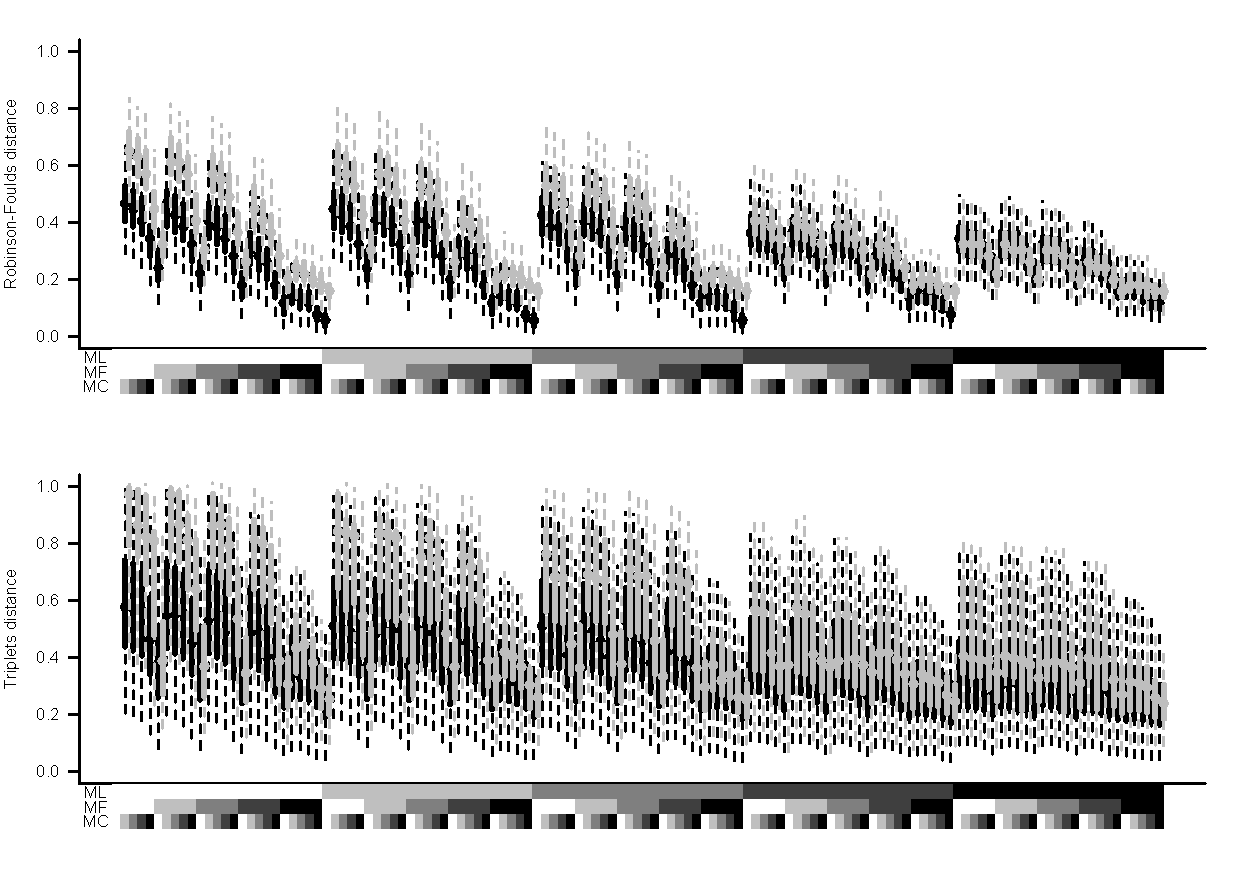
\includegraphics[width=1\textwidth]{SupplementaryMaterial/Supp_Figures/Boot+Baytre-AllParam-RF+Tr.pdf}
\caption{Trend of the effect of missing data on topological recovery on the Bootstraps and the Bayesian posterior trees distributions. The amount of missing data per parameter ($M_{L}$, $M_{F}$ and $M_{C}$) is represented along the x axis. The colour gradient from white to black represents respectively, 0\%, 10\%, 25\%, 50\% and 75\% of missing data. The topological recovery is represented on the y axis, both using Robinson-Foulds distance (upper row) and Triplets distance (lower row). Points represent the modal value of each distribution ; thick solid and thin dashed lines represents respectively the 50\% and 95\% confidence intervals or the distributions. The Bootstraps are represented in black and the Bayesian posterior trees distributions in grey.}
\label{Fig_global_BootTreesets} %Differences between all the parameters and between two methods (Boot vs treesets)
\end{figure}

\begin{figure} 
\centering
    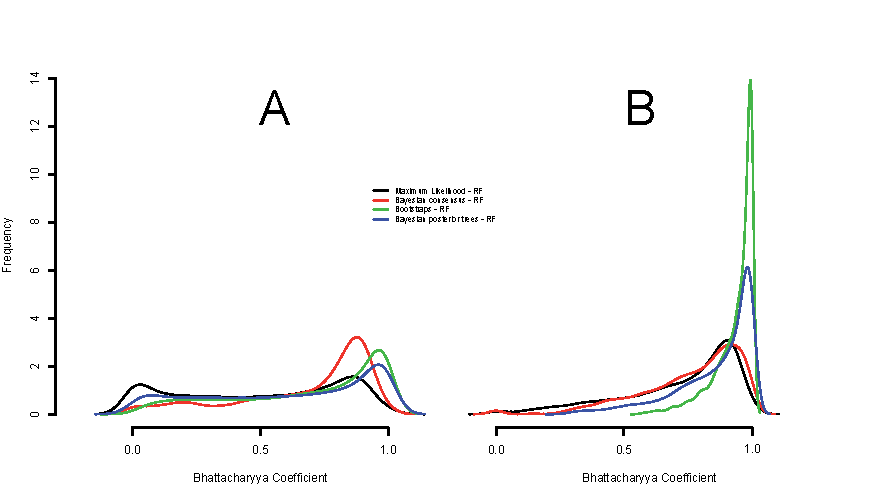
\includegraphics[width=1\textwidth]{SupplementaryMaterial/Supp_Figures/BC-AllMethods-RF+Tr.pdf}
\caption{Distribution of the Pairwise Bhattacharyya Coefficients within each method. A- Distribution of the coefficients when comparing Ronbinson-Foulds distances. B- Distribution of the coefficients when comparing Triplets distances.}
\label{Fig_Bhatt.coeff_distribution} %Differences in overlap within each method
\end{figure}

\begin{figure} 
\centering
    \includegraphics[width=1\textwidth]{SupplementaryMaterial/Supp_Figures/PairwiseComp-ML-RF+Tr.pdf}
\caption{Pairwise Bhattacharyya Coefficients within the Maximum Likelihood trees. The pairwise trees comparisons are represent on both axis. The colour gradient from white to black represents respectively, 0\%, 10\%, 25\%, 50\% and 75\% of missing data for each parameter. The matrix represents the values of pairwise Bhattacharyya Coefficients going from green (1) to red (0). A. Results for the Normalised Robinson-Foulds distance. B. Results with the for Normalised Triplets distance.}
\label{Fig_pairComp-Baytree-RF}
\end{figure} %Pairwise BC for the ML for RF+Tr. (parameters differences)

\begin{figure} 
\centering
    \includegraphics[width=1\textwidth]{SupplementaryMaterial/Supp_Figures/PairwiseComp-Boot-RF+Tr.pdf}
\caption{Pairwise Bhattacharyya Coefficients within the Bootstrap trees. The pairwise trees comparisons are represent on both axis. The colour gradient from white to black represents respectively, 0\%, 10\%, 25\%, 50\% and 75\% of missing data for each parameter. The matrix represents the values of pairwise Bhattacharyya Coefficients going from green (1) to red (0). A. Results for the Normalised Robinson-Foulds distance. B. Results with the for Normalised Triplets distance.}
\label{Fig_pairComp-Baytree-Tr}
\end{figure} %Pairwise BC for the Boot for RF+Tr. (parameters differences)

\begin{figure} 
\centering
    \includegraphics[width=1\textwidth]{SupplementaryMaterial/Supp_Figures/PairwiseComp-Baytre-RF+Tr.pdf}
\caption{Pairwise Bhattacharyya Coefficients within the Bayesian posterior distribution trees. The pairwise trees comparisons are represent on both axis. The colour gradient from white to black represents respectively, 0\%, 10\%, 25\%, 50\% and 75\% of missing data for each parameter. The matrix represents the values of pairwise Bhattacharyya Coefficients going from green (1) to red (0). A. Results for the Normalised Robinson-Foulds distance. B. Results with the for Normalised Triplets distance.}
\label{Fig_pairComp-MLbest-RF}
\end{figure} %Pairwise BC for the Baytre for RF+Tr. (parameters differences)


%Summary of metrics values for all parameters combinations
\begin{table}[ht]
\centering
\begin{tabular}{rrrrrrr}
  \hline
 & Min. & 1st Qu. & Median & Mean & 3rd Qu. & Max. \\ 
  \hline
  Maximum likelihood-RF & 0.06 & 0.26 & 0.40 & 0.41 & 0.50 & 0.95 \\ 
  Maximumlikelihood-Tr & 0.29 & 0.45 & 0.59 & 0.63 & 0.84 & 1.00 \\ 
  Bayesian consensus-RF & 0.69 & 0.71 & 0.72 & 0.76 & 0.79 & 0.96 \\ 
  Bayesian consensus-Tr & -0.28 & -0.11 & 0.17 & 0.19 & 0.37 & 0.98 \\ 
  Bootstraps-RF & 0.06 & 0.18 & 0.27 & 0.26 & 0.34 & 0.46 \\ 
  Bootstraps-Tr & 0.23 & 0.31 & 0.35 & 0.38 & 0.45 & 0.58 \\ 
  Bayesian posterior trees-RF & 0.16 & 0.22 & 0.32 & 0.34 & 0.42 & 0.65 \\ 
  Bayesian posterior trees-Tr & 0.24 & 0.35 & 0.40 & 0.50 & 0.67 & 0.98 \\ 
   \hline
   \hline
\end{tabular}
\end{table}

%Summary of metrics values for the ML parameter
\begin{table}[ht]
\centering
\begin{tabular}{rrrrrrr}
  \hline
 & Min. & 1st Qu. & Median & Mean & 3rd Qu. & Max. \\ 
  \hline
Maximum likelihood-RF & 0.44 & 0.51 & 0.63 & 0.66 & 0.78 & 0.95 \\ 
  Maximumlikelihood-Tr & 0.45 & 0.56 & 0.76 & 0.74 & 0.93 & 0.99 \\ 
  Bayesian consensus-RF & 0.71 & 0.73 & 0.80 & 0.82 & 0.88 & 0.95 \\ 
  Bayesian consensus-Tr & 0.37 & 0.46 & 0.67 & 0.67 & 0.87 & 0.96 \\ 
  Bootstraps-RF & 0.34 & 0.37 & 0.42 & 0.41 & 0.44 & 0.46 \\ 
  Bootstraps-Tr & 0.32 & 0.40 & 0.51 & 0.46 & 0.51 & 0.57 \\ 
  Bayesian posterior trees-RF & 0.33 & 0.41 & 0.52 & 0.50 & 0.60 & 0.65 \\ 
  Bayesian posterior trees-Tr & 0.41 & 0.56 & 0.76 & 0.71 & 0.84 & 0.98 \\ 
   \hline
\end{tabular}
\end{table}

%Summary of metrics values for the ML parameter
\begin{table}[ht]
\centering
\begin{tabular}{rrrrrrr}
  \hline
 & Min. & 1st Qu. & Median & Mean & 3rd Qu. & Max. \\ 
  \hline
Maximum likelihood-RF & 0.23 & 0.46 & 0.64 & 0.61 & 0.79 & 0.93 \\ 
  Maximumlikelihood-Tr & 0.65 & 0.84 & 0.95 & 0.89 & 0.99 & 1.00 \\ 
  Bayesian consensus-RF & 0.72 & 0.77 & 0.86 & 0.85 & 0.94 & 0.96 \\ 
  Bayesian consensus-Tr & -0.16 & 0.19 & 0.63 & 0.52 & 0.96 & 0.98 \\ 
  Bootstraps-RF & 0.14 & 0.30 & 0.40 & 0.35 & 0.45 & 0.46 \\ 
  Bootstraps-Tr & 0.37 & 0.49 & 0.54 & 0.51 & 0.56 & 0.57 \\ 
  Bayesian posterior trees-RF & 0.24 & 0.45 & 0.57 & 0.51 & 0.63 & 0.65 \\ 
  Bayesian posterior trees-Tr & 0.44 & 0.81 & 0.86 & 0.82 & 0.98 & 0.98 \\ 
   \hline
\end{tabular}
\end{table}

%Summary of metrics values for the MC parameter
\begin{table}[ht]
\centering
\begin{tabular}{rrrrrrr}
  \hline
 & Min. & 1st Qu. & Median & Mean & 3rd Qu. & Max. \\ 
  \hline
Maximum likelihood-RF & 0.40 & 0.50 & 0.64 & 0.65 & 0.79 & 0.94 \\ 
  Maximumlikelihood-Tr & 0.70 & 0.84 & 0.93 & 0.89 & 0.99 & 1.00 \\ 
  Bayesian consensus-RF & 0.76 & 0.79 & 0.86 & 0.86 & 0.92 & 0.96 \\ 
  Bayesian consensus-Tr & 0.05 & 0.16 & 0.53 & 0.50 & 0.87 & 0.92 \\ 
  Bootstraps-RF & 0.25 & 0.34 & 0.42 & 0.38 & 0.45 & 0.46 \\ 
  Bootstraps-Tr & 0.38 & 0.47 & 0.55 & 0.51 & 0.57 & 0.58 \\ 
  Bayesian posterior trees-RF & 0.32 & 0.44 & 0.58 & 0.52 & 0.62 & 0.65 \\ 
  Bayesian posterior trees-Tr & 0.39 & 0.78 & 0.82 & 0.79 & 0.98 & 0.98 \\ 
   \hline
\end{tabular}
\end{table}


%Summary of the BC between pairs of methods for the ML parameter
\begin{table}[ht]
\centering
\begin{tabular}{rrrrrrr}
  \hline
 & Min. & 1st Qu. & Median & Mean & 3rd Qu. & Max. \\ 
  \hline
Maximum.likelihood.vs..Bayesian.consensus...RF & 0.30 & 0.31 & 0.69 & 0.61 & 0.77 & 1.00 \\ 
  Maximum.likelihood.vs..Bayesian.consensus...Tr & 0.79 & 0.81 & 0.84 & 0.86 & 0.85 & 1.00 \\ 
  Maximum.likelihood.vs..Bootstraps...RF & 0.03 & 0.22 & 0.29 & 0.36 & 0.54 & 0.69 \\ 
  Maximum.likelihood.vs..Bootstraps...Tr & 0.08 & 0.42 & 0.53 & 0.51 & 0.74 & 0.78 \\ 
  Maximum.likelihood.vs..Bayesian.posterior.trees...RF & 0.02 & 0.49 & 0.61 & 0.51 & 0.67 & 0.74 \\ 
  Maximum.likelihood.vs..Bayesian.posterior.trees...Tr & 0.21 & 0.61 & 0.70 & 0.63 & 0.81 & 0.81 \\ 
  Bayesian.consensus.vs..Bootstraps...RF & 0.01 & 0.02 & 0.02 & 0.02 & 0.03 & 0.04 \\ 
  Bayesian.consensus.vs..Bootstraps...Tr & 0.08 & 0.69 & 0.78 & 0.64 & 0.79 & 0.84 \\ 
  Bayesian.consensus.vs..Bayesian.posterior.trees...RF & 0.01 & 0.02 & 0.02 & 0.04 & 0.08 & 0.09 \\ 
  Bayesian.consensus.vs..Bayesian.posterior.trees...Tr & 0.21 & 0.74 & 0.75 & 0.68 & 0.84 & 0.87 \\ 
  Boostraps.vs..Bayesian.posterior.trees...RF & 0.69 & 0.75 & 0.85 & 0.85 & 0.95 & 1.00 \\ 
  Boostraps.vs..Bayesian.posterior.trees...Tr & 0.91 & 0.92 & 0.96 & 0.95 & 0.97 & 0.98 \\ 
   \hline
\end{tabular}
\end{table}

%Summary of the BC between pairs of methods for the MF parameter
\begin{table}[ht]
\centering
\begin{tabular}{rrrrrrr}
  \hline
 & Min. & 1st Qu. & Median & Mean & 3rd Qu. & Max. \\ 
  \hline
Maximum.likelihood.vs..Bayesian.consensus...RF & 0.00 & 0.25 & 0.48 & 0.50 & 0.76 & 1.00 \\ 
  Maximum.likelihood.vs..Bayesian.consensus...Tr & 0.38 & 0.69 & 0.75 & 0.72 & 0.80 & 1.00 \\ 
  Maximum.likelihood.vs..Bootstraps...RF & 0.03 & 0.18 & 0.32 & 0.36 & 0.47 & 0.77 \\ 
  Maximum.likelihood.vs..Bootstraps...Tr & 0.08 & 0.34 & 0.40 & 0.38 & 0.53 & 0.55 \\ 
  Maximum.likelihood.vs..Bayesian.posterior.trees...RF & 0.02 & 0.47 & 0.71 & 0.60 & 0.86 & 0.94 \\ 
  Maximum.likelihood.vs..Bayesian.posterior.trees...Tr & 0.21 & 0.54 & 0.62 & 0.56 & 0.64 & 0.80 \\ 
  Bayesian.consensus.vs..Bootstraps...RF & 0.00 & 0.00 & 0.01 & 0.01 & 0.01 & 0.03 \\ 
  Bayesian.consensus.vs..Bootstraps...Tr & 0.08 & 0.38 & 0.54 & 0.49 & 0.70 & 0.75 \\ 
  Bayesian.consensus.vs..Bayesian.posterior.trees...RF & 0.00 & 0.02 & 0.02 & 0.02 & 0.04 & 0.04 \\ 
  Bayesian.consensus.vs..Bayesian.posterior.trees...Tr & 0.21 & 0.29 & 0.66 & 0.54 & 0.72 & 0.82 \\ 
  Boostraps.vs..Bayesian.posterior.trees...RF & 0.69 & 0.69 & 0.72 & 0.71 & 0.72 & 0.72 \\ 
  Boostraps.vs..Bayesian.posterior.trees...Tr & 0.91 & 0.91 & 0.91 & 0.93 & 0.92 & 0.98 \\ 
   \hline
\end{tabular}
\end{table}

%Summary of the BC between pairs of methods for the MC parameter
\begin{table}[ht]
\centering
\begin{tabular}{rrrrrrr}
  \hline
 & Min. & 1st Qu. & Median & Mean & 3rd Qu. & Max. \\ 
  \hline
Maximum.likelihood.vs..Bayesian.consensus...RF & 0.03 & 0.32 & 0.66 & 0.55 & 0.75 & 1.00 \\ 
  Maximum.likelihood.vs..Bayesian.consensus...Tr & 0.51 & 0.69 & 0.80 & 0.76 & 0.80 & 1.00 \\ 
  Maximum.likelihood.vs..Bootstraps...RF & 0.03 & 0.17 & 0.21 & 0.31 & 0.46 & 0.68 \\ 
  Maximum.likelihood.vs..Bootstraps...Tr & 0.08 & 0.31 & 0.39 & 0.39 & 0.56 & 0.61 \\ 
  Maximum.likelihood.vs..Bayesian.posterior.trees...RF & 0.02 & 0.44 & 0.47 & 0.52 & 0.78 & 0.90 \\ 
  Maximum.likelihood.vs..Bayesian.posterior.trees...Tr & 0.21 & 0.52 & 0.59 & 0.55 & 0.66 & 0.77 \\ 
  Bayesian.consensus.vs..Bootstraps...RF & 0.00 & 0.01 & 0.01 & 0.02 & 0.02 & 0.03 \\ 
  Bayesian.consensus.vs..Bootstraps...Tr & 0.08 & 0.47 & 0.62 & 0.51 & 0.66 & 0.73 \\ 
  Bayesian.consensus.vs..Bayesian.posterior.trees...RF & 0.00 & 0.02 & 0.04 & 0.04 & 0.05 & 0.06 \\ 
  Bayesian.consensus.vs..Bayesian.posterior.trees...Tr & 0.21 & 0.45 & 0.64 & 0.57 & 0.74 & 0.79 \\ 
  Boostraps.vs..Bayesian.posterior.trees...RF & 0.69 & 0.73 & 0.73 & 0.76 & 0.81 & 0.86 \\ 
  Boostraps.vs..Bayesian.posterior.trees...Tr & 0.91 & 0.92 & 0.93 & 0.94 & 0.96 & 0.99 \\ 
   \hline
\end{tabular}
\end{table}
  \label{Supp_results}

%END
\end{document}
    \label{SupplementaryMaterial}

%END
\end{document}